


\begin{abstract}[\hspace*{-10pt}]
    This chapter draws mainly on the submitted work: \fullcite{van_biesbroeck_robust_2025}  % Ce chapitre reprend principalement les travaux publiés dans: 
\end{abstract}

\begin{abstract}
    To estimate seismic fragility curves using the Bayesian framework,
    the observed data constitute the most objective source of information to consider.
    % information that comes from the data represents 
    In this chapter, we conduct a Bayesian estimation of seismic fragility curves that aims to optimize that information. We consider datasets that have the disadvantages of (i) being scarce, and (ii) reducing structural responses to binary outcomes. However, we propose an experimental design that is sought to select seismic signals that are expected to maximize the impact of  data on the posterior distribution.
    Moreover, our approach is supported by the reference prior theory, to ensure the prior itself maximizes the influence of  data on the posterior.
    The reference prior is slightly constrained in this work in order to tackle occurrences of so-called degenerate likelihoods.
    % that are ubiquitous with small data sets.
%    This strategy aims to maximize the impact of the  data on the posterior distribution of the fragility curve {and its strength is to extend to any prior of interest, provided it is proper}. Our method is applied to a case study of the nuclear industry. 
The results demonstrate the ability of the method to efficiently and robustly estimate fragility curves, and to avoid degeneracy even with limited data. Additionally, we demonstrate that the estimates quickly reach the model bias induced by the probit-lognormal modeling. % that we implement. %{Two criteria are suggested to help the user stop the experiment design algorithm.}
\end{abstract}


\minitoc

\section{Introduction}


In this chapter, we conduct a Bayesian estimation of seismic fragility curves. Seismic fragility curves, which are defined as the probability of failure of a mechanical equipment conditional to a given intensity measure (IM) of the seismic scenario, are reviewed in \cref{chap:frags-intro}. We continue to focus on case studies where (i) the information about the structure's response is limited to a binary outcome (i.e., failure or non-failure) and (ii) the available data are scarce. 

In the Bayesian workflow, two sources of information are combined to issue the posterior distribution, which provides estimates of the quantities of interest. 
Specifically, \emph{a priori} information  coexists with information that comes from the observations, and that is incorporated through the statistical model.
%Regarding seismic fragility curves estimation, we elucidated in \cref{chap:prem} and \cref{chap:constrained-frags} how the first one can be constructed to issue consistent and accurate estimations of the curves.

This thought is fundamental %as a cornerstone 
when it resorts to estimating seismic fragility curves.
Indeed, the developments done in \cref{chap:prem} and \cref{chap:constrained-frags}
have shown that (i)~the \emph{a priori} information  must be carefully defined, since any  subjectivity embedded into its design may significantly impact the estimates, and (ii)~the information that comes from the data can take ``degenerate'' forms, jeopardizing efficiency.
%it embedds
%Indeed, we elucidated in \cref{chap:prem} and \cref{chap:constrained-frags} how the information \emph{a priori} can be arranged to.
In these chapters, we proved that appropriate prior designs can yield accurate estimates of seismic fragility curves
%  Those being unaffected by degenerate scenarios if a relevant constraints
% the prior can be designed in a way that 
% permits accurate estimations of seismic fragility curves, 
without being affected by degenerate scenarios. These appropriate priors 
correspond to constrained reference priors, where the constraints are sought to regularize the decay rates of the objective Jeffreys prior in order to ensure it yields proper posteriors.
% take the form of reference priors to which
% correspond to reference priors that are 
%proved how t
% We proved that the first one can be designed 
Nevertheless, the influence of data on the posterior remains important. %influence on the estimates. %The more the data are close to a degeneracy, the %more 
%less the posterior
In practice, %two datasets of the same size do not contain the same amount of knowledge, and one will inform more the posterior than the other. 
%Optimizing that information will inevitably guide the result away from the prior, enhancing objectivity as well.
two datasets of the same size may differ considerably in the information they convey, with one contributing more effectively to the posterior than the other. Enhancing this contribution will inevitably guide the result ``aside'' from the prior, which will improve objectivity as well.
% can improve objectivity and reduce reliance on prior assumptions.


% the posterior distribution resembles to the prior. If the latter is sought to minimize subjectivity, then it must be low



% When the latter is degenerate, the prior information takes 
%Two 


In this chapter, we propose a strategy of design of experiments (DoE), to get the most out of the probit-lognormal model, namely the most accurate and robust estimation possible with the minimum of data. Given a large database of synthetic seismic signals ---generated to match the seismic scenario of interest--- the proposed strategy intends to sequentially select the synthetic signals with which to perform 
%the calculations or 
the tests, in order to optimally estimate ---by minimizing their number--- the probit-lognormal estimations of fragility curves. 
Different strategies exist to conduct an experimental design. Generally, they are based on the definition of a criterion, such as the stepwise uncertainty reduction (SUR) one, introduced by \citet{villemonteix_informational_2009}. 
As for examples of studies in reliability analysis that conduct a criterion-based experimental design, we can cite \cite{bect_supermartingale_2019,azzimonti_adaptive_2021,agrell_sequential_2021,lartaud_sequential_2025}.
%The most common are based on 
%In reliability analysis, it is common to refer to techniques that are based 
%Experimental designs are common in reliability analysis
Our work proposes a strategy inherited from the reference prior theory, i.e., based on the information theory. We recall that the reference prior theory is introduced in \cref{chap:intro-ref}. This strategy aims to maximize the impact that the selected data has on the posterior distribution of the fragility curve. 
This paradigm is not only used to construct an objective prior, %ensuring its objectivity, 
but also to define a criterion from which is based our experimental design.





It is also important to recognize that the model itself provides information to the Bayesian workflow and influences the posterior.
For instance, 
we draw attention to the work conducted in \cref{app:chap:ESAIM}, where a simple model that assumes a linear correlation between the logarithm of the structural response and that of the IM is implemented with a similar experimental design. 
%The results presented in this appendix illustrate the possible limitations of models that lead to estimation biases whose “importance” depends on the assumptions considered.
The results presented in that appendix illustrate the possible limitations of models that lead to estimation biases whose  highlight the limitations of the model,  entailed by its irreducible bias. % and resulting to biased estimates. 
In this chapter, we acknowledge that the probit-lognormal model %that we implement in this chapter 
is itself inherently biased. However, we aim to demonstrate that this model can accurately estimate seismic fragility curves in scenarios with limited data if used as part of an approach built on a full understanding of the model's limitations.
%



%as said earlier, the information that comes from the data is embedded in the Bayesian workflow through the implemented statistical model.
%This means the latter has its own influence on the estimates. In \cref{app:chap:ESAIM} a simple model that assumes a linear correlation between the logarithm of the structural response and that of the IM is implemented with a similar experimental design.




% While we recognize that the model admits an irreducible biais 

% is limited 
% the probit-lognormal model is 



% In our framework,
% we do not change the probit-lognormal modeling of the fragility curve.




%In this framework, this work addresses problems for which a limited amount of binary data is available. In this sense, this paper mainly addresses equipment problems for which only binary results of seismic tests are available (e.g., qualification tests of electrical relay, etc.) or also simulation-based approaches whose results are restricted to binary data. These latter situations are encountered in practice when the amount of available data is limited, because fitting sophisticated statistical models may require a larger amount of data to be relevant. 
% For instance, in \cite{mai_seismic_2017} and \cref{app:chap:ESAIM} the authors showed that the simplest model that assumes a linear correlation between the logarithm of the structural response of interest and the logarithm of the IM should be avoided because of the irreducible model bias that this can entail and which can greatly affect the estimation of the fragility curves. 


{Finally, note that the strategy proposed in this chapter echoes the conclusions of the recent reference \mbox{\cite{zhu_seismic_2023}}. In this reference, it is indeed recommended to use adaptive strategies to deal with problems involving high failure thresholds, even with the use of more sophisticated models than the probit-lognormal model. We show here that this conclusion obviously applies to the probit-lognormal model. Our strategy therefore allows us to extend its domain of validity, by exploiting it as best we can whatever the failure threshold of interest.}



The rest of the chapter is organized as follows. In the next section we start by briefly recalling the probit-lognormal modeling of fragility curves, and we 
present the constrained priors that we propose.
The experimental design is explained and detailed in \cref{sec:doe:PEmethod}, and benchmarking metrics that serve to evaluate the performances of our approach are defined in \cref{sec:doe:metrics}. 
The method is then implemented on a case study in \cref{sec:doe:application}, where a thorough analysis of our results is conducted.
In order to provide more insights about the behavior of the DoE, we suggest another implementation of the method on toy case studies in \cref{app:doe:toycases}. Finally, a conclusion terminates this chapter in \cref{sec:doe:conclusion}.






\section{Probit-lognormal modeling and constrained reference prior}\label{sec:doe:model}

We recall briefly the probit-lognormal model that was introduced in \cref{chap:frags-intro}. We suppose to observe realizations of the random vector $(Z,A)$, where $A\in\cA\subset(0,\infty)$ represents the IM value, and $Z\in\{0,1\}$ represents the binary outcome ($Z=1$ if the equipment fails and $Z=0$ otherwise).
The probit-lognormal model consist in assuming the following parameterized distribution of $(Z,A)$ conditionally to the parameter $\theta=(\alpha,\beta)=\Theta=(0,\infty)^2$:
    \begin{equation}
        A\sim A|\theta\sim H,\quad\text{and}\quad Z|A,\theta\sim\cB(P_f(A))\quad\text{with}\quad P_f(a)=\Phi\left(\frac{\log a-\log\alpha}{\beta}\right),
    \end{equation}
where $\cB$ refers to a Bernoulli distribution, and $H$ is the distribution of $A$, its density is $h$. %and $\Phi$ to the c.d.f. of a standard Gaussian.
Given observations $\mbf z^k=(z_i)_{i=1}^k$, $\mbf a^k=(a_i)_{i=1}^k$, the likelihood of this model is the following:
    \begin{equation}
        \ell_k(\mbf z^k|\mbf a^k,\theta) = \prod_{i=1}^{k}\ell(z_i|a_i,\theta) = \prod_{i=1}^k\Phi\left(\frac{\log a_i-\log\alpha}{\beta}\right)^{z_i}\left(1-\Phi\left(\frac{\log a_i-\log\alpha}{\beta}\right)\right)^{z_i}.
    \end{equation}
The decay rates of this likelihood vary significantly as a function of the observations. We remind below the definition of a degenerate likelihood that we introduced in \cref{chap:prem}, where the decay rates of the likelihood were comprehensively studied.

\begin{defistarred}[Likelihood degeneracy; reminder of \cref{def:degeneracy}] %\label{def:doe:degeneracy}
    %If the observed data $(\mbf z^k,\mbf a^k)$ are such that, either,
    If the observed samples $(\mbf z^k,\mbf a^k)$ belong to one of the following three types:
    \begin{itemize}
        \item
        type 1 : no failure is observed: $z_i=0$ for any $i$;
        \item type 2 : only failures are observed: $z_i=1$ for any $i$;
        \item type 3 : the failures and non-failures are partitioned into two disjoint subsets when classified according to their IM values:
        %the failures and successes are discriminated according to their IM: 
        there exists $a\in\cA$ such that for any $i,j$, $a_i<a<a_j\Longleftrightarrow z_i\ne z_j$; % (see the illustration in \cref{fig:constr-frags:degenerate-frag});
    \end{itemize}
    then the likelihood is degenerate.
\end{defistarred}




To conduct a Bayesian estimation of probit-lognormal fragility curves, one should select a prior carefully to ensure it issues a proper posterior even in degenerate scenarios. We define below adequate requirements for a robust \emph{a posteriori} estimation, i.e., an estimation that results from a proper posterior.

\begin{defi}[Robust \emph{a posteriori} estimation]\label{def:doe:robust-estimation}
    The \emph{a posteriori} estimation is called robust if the posterior is proper. For  seismic fragility curves it is the case if:
    \begin{itemize}
        \item the likelihood is not degenerate and the prior verifies
            \begin{align*}
                &\forall\beta>0,\,\pi(\theta)\aseq{\log\alpha\rightarrow\pm\infty}O(1),\\
                & \forall\alpha>0,\,\pi(\theta)\aseq{\beta\rightarrow0} O(1),\quad\text{and}\quad \pi(\theta)\ \text{is integrable in the neighborhood of $\beta\to\infty$.}
            \end{align*}
        \item the likelihood is degenerate, the prior is proper w.r.t $\beta$ and verifies $\forall\beta>0,\, \pi(\theta)\aseq{\log\alpha\rightarrow\pm\infty}O(1)$.
    \end{itemize}
\end{defi}


In this chapter, we select a prior that is supported by the reference prior theory, in order to minimize its subjectivity.
%To conduct a Bayesian estimation of , we construct a prior by taking the reference prior theory as a support.
We remind that the theory is reviewed and developed in the \cref{part:ref-theory} of this manuscript. %Also, we refer to the development 
In \cref{chap:prem} a reference prior that takes the form of a Jeffreys prior was derived and studied in the context of probit-lognormal fragility curves.
This prior being inefficient in degenerate scenario, one constraint was proposed in \cref{chap:constrained-frags} to circumvent this problem.
The prior approached in that work was given by the density:
    \begin{equation}\label{eq:doe:trueconstrref}
        \pi_\gamma(\theta)\propto J(\theta)\beta^\gamma,\quad\text{where}\quad \gamma\in(0,2).
    \end{equation}
The same approach is conducted here, where we propose a novel prior that is more computationally efficient. Indeed, since the prior will be evaluated multiple time to provide \emph{a posteriori} estimates using Markov chain Monte Carlo (MCMC) techniques, we aim to suggest a prior that is not expensive to evaluate.
That prior, which has a density that we denote $\pi^\ast_\gamma$, is sought to resemble to the properly constrained reference prior expressed in \cref{eq:doe:trueconstrref}:
    \begin{equation}\label{eq:doe:tilde-pi-gamma}
        \pi^\ast_\gamma(\theta) \propto\frac{1}{\alpha(\beta^{1-\gamma}+\beta^{3-\gamma})}\exp\left(-\frac{(\log\alpha-\mu_A)^2}{2\sigma_A^2+2\beta^2}\right),
    \end{equation}
    where $\mu_A$ and $\sigma_A$ respectively denote the mean and the standard deviation of the r.v. $\log A$.
The form of the prior density $\pi^\ast_\gamma$ results partly from the consideration of Jeffreys prior's decay rates. With respect to $\beta$, the decay rates are the same as the ones of the constrained reference prior density in \cref{eq:doe:trueconstrref} (see the study of Jeffreys prior's decays in \cref{chap:prem}, \cref{sec:PREM:subsec:jeffasymp}). With respect to $\alpha$, the prior density $\pi^\ast_\gamma$ admits slightly different decay rates (a term equivalent to $|\log\alpha|$ vanished). That choice results from two considerations: (i)~especially outside degenerate likelihoods of types 1 or 2, this change has a negligible impact on the posterior, and (ii)~in \cref{chap:prem} (\cref{sec:PREM:subsec-jeffprectical}) we elucidated that the reference prior w.r.t. $\alpha$ is close to the distribution of the IM, which is associated to a log-normal distribution.
We precise that both priors in \cref{eq:doe:trueconstrref,eq:doe:tilde-pi-gamma} have been tested when we conducted our numerical results to ensure they give non-distinguishable results.

% similar to the form the Jefr


While $0<\gamma<2$, the prior satisfies both criteria required for a robust \emph{a posteriori} estimation (\cref{def:doe:robust-estimation}). The case $\gamma=0$ corresponds to the critical case where $\pi^\ast_\gamma$ is similar to the Jeffreys prior density and thus provides a robust \emph{a posteriori} estimation if and only if the likelihood is not degenerate. The limit case $\gamma=2$ never provides a robust \emph{a posteriori} estimation. We precise that the methodology presented in the next section requires that the prior tackles degenerate-likelihood cases. The tuning of this hyper-parameter must be thought as the research for a balance between objectivity ($\gamma$ closer to $0$) and suitability for inference. The influence of $\gamma$ is studied in the practical application of our method in \cref{sec:doe:application}.




%  that reference prior is constrained







\section{Sequential design of experiments% based on a proper objective prior
}\label{sec:doe:PEmethod}

\subsection{Methodology description}



The priors defined in \cref{eq:doe:tilde-pi-gamma} handle the degeneracy of the likelihood to provide robust \emph{a posteriori} estimation of the fragility curve. However, it remains important to reduce the occurrence of this phenomenon because: %even if  astonished
%they are in any way representative of a lack of information
    \begin{enumerate}
        \item[(i)]  even if it partially disappears thanks to the slightly informed priors we suggest, { the possibility of obtaining estimates that tend towards unrealistic fragility curves always exists with very small data sizes;}
        \item[(ii)] by nature, a likelihood becomes degenerate consequently to a lack of information within the observed data samples. Extinguishing degeneracy should thus lead to a better understanding of the structure's response and its fragility curve.
    \end{enumerate}

In this chapter, we propose to tackle degeneracy with an appropriate experimental design strategy. 
Different sequential methods exist. Suppose that we have observed the sample $(\mbf z^k,\mbf a^k)$, we need to create a criterion to choose the next input $a_{k+1}$. 
Given our analysis (statement (ii) above) from an information theory viewpoint, the strategy to build this criterion is to maximize the impact that the selected observation would have on the posterior distribution. 
This strategy echoes the one that supports the reference prior definition as a maximal argument of the mutual information, so that we suggest a similar criterion to select $a_{k+1}$:
      \begin{equation}\label{eq:doe:index}
        a_{k+1}=\argmax_{a\in\cA}\cI_{k+1}(a);\quad 
            \cI_{k+1}(a_{k+1}) = \EE_{{z_{k+1}}|\mbf a^{k+1},\mbf z^k}[D_\delta(p(\theta|\mbf z^k,\mbf a^k)||p(\theta|\mbf z^{k+1},\mbf a^{k+1}))].
    \end{equation}
The index $\cI_{k+1}$ can be seen as a sensitivity index measuring the sensitivity of the posterior w.r.t. the data \citep{da_veiga_global_2015}. Its sequential maximization amounts to maximize the impact of the data to the posterior. %the sensitivity of estimates of $\theta$ w.r.t. the observations.
Our index can be seen as derived from the popular framework of Stepwise Uncertainty Reduction techniques \citep{villemonteix_informational_2009}. %\citep{bect_supermartingale_2019}. 
Typically,  those methods are formulated with an \emph{a posteriori} variance within the expectation in \cref{eq:doe:index} instead of the dissimilarity measure suggested here.
\Cref{alg:doe:PE} proposes a practical pseudo-code of our methodology. It requires to derive an approximation of the index $\cI_{k+1}$, which we elucidate in the following section.




% \newcommand{\algorithmicreinit}{\textbf{Init:}}

\renewcommand{\algorithmicrequire}{\textbf{Notations:}}

 \begin{algorithm*}
		\caption{Planning of experiments}
		\begin{algorithmic}
            % \STATE \textbf{INIT:}
            \REQUIRE \begin{tabular}[t]{l}
			Seismic signal : $\cS$\\ Intensity measure of the seismic signal: $\mathrm{IM}(\cS)$\\ Mechanical response to the seismic signal (failure or success): $\mathrm R(\cS)$ 
			\end{tabular}\renewcommand{\algorithmicrequire}{\textbf{Initialization:}}
            \REQUIRE \begin{tabular}[t]{l}
			$k_0>0$ (in practice $k_0=2$), initial seismic signals $\cS_1,\dots,\cS_{k_0}$\\
            Define the initial data: $\mbf z^{k_0}=(\mathrm{R}(\cS_1),\dots,\mathrm{R}(\cS_{k_0})),\   \mbf a^{k_0}=(\mathrm{IM}(\cS_1),\dots,\mathrm{IM}(\cS_{k_0}))$
			\end{tabular}
            \FOR{$k=k_0\dots k_{\text{max}}-1$ }
	            \STATE Approximate $\cI_{k+1}$ via Monte Carlo sampling
                \STATE Compute $a_{k+1}=\argmax_a\cI_{k+1}(a)$
	            \STATE Choose a seismic signal $\cS_{k+1}$ such that $\mathrm{IM}(\cS_{k+1})=a_{k+1}$
                \STATE {Perform the %numerical calculation or 
                experiment and} define $z_{k+1}=\mathrm{R}(\cS_{k+1})$
	        \ENDFOR
		\end{algorithmic}
	    \label{alg:doe:PE}
	\end{algorithm*}


\subsection{Approximation of the index}
%{!! Il y a des variations de notation : $a_{k+1}$ vs. $a^{k+1}$ !!}

Let us adopt the short notation
    \begin{equation}
        \Psi^z_a(\theta)=\Phi\left(\frac{\log a-\log\alpha}{\beta}\right)^z\left(1-\Phi\left(\frac{\log a-\log\alpha}{\beta}\right)\right)^{1-z}.
    \end{equation}
The index to maximize has the following form:
    \begin{align}
        \cI_{k+1}(a_{k+1})&= (\delta(\delta-1))^{-1}
            \sum_{z\in\{0,1\}}
                \PP({z_{k+1}}=z|\mbf a^{k+1},\mbf z^{k})
                \Delta_{k+1}(\mbf a^{k+1},\mbf z^{k+1})
    \end{align}
with :
    %\begin{align}
        $\PP({z_{k+1}}=z|\mbf a^{k+1},\mbf z^{k+1}) = \int_{\Theta}\Psi^{z}_{a_{k+1}}(\theta)p(\theta|\mbf z^{k},\mbf a^{k})d\theta,$
    %\end{align}
and,
    \begin{align}
        \Delta_{k+1}(\mbf a^{k+1},\mbf z^{k+1}) &=
            \int_{\Theta}\left(\frac{p(\theta|\mbf z^{k},\mbf a^{k})}{p(\theta|\mbf z^{k+1},\mbf a^{k+1})}\right)^{\delta}p(\theta|\mbf z^{k+1},\mbf a^{k+1})d\theta \nonumber\\
        &=\int_\Theta \left(\frac{\int_\Theta p(\vartheta|\mbf z^k,\mbf a^k)\Psi^{z_{k+1}}_{a_{k+1}}(\vartheta)d\vartheta}{\Psi^{z_{k+1}}_{a_{k+1}}(\theta) } \right)^\delta \frac{\Psi^{z_{k+1}}_{a_{k+1}}(\theta)p(\theta|\mbf z^k,\mbf a^k) }{\int_\Theta p(\vartheta|\mbf z^k,\mbf a^k)\Psi^{z_{k+1}}_{a_{k+1}}(\vartheta)d\vartheta} d\theta\\
        &= \left(\int_\Theta \Psi^{z_{k+1}}_{a_{k+1}}(\theta) p(\theta| \mbf z^k, \mbf a^k) d\theta\right)^{\delta-1}  \int_\Theta \Psi^{z_{k+1}}_{a_{k+1}}(\theta)^{1-\delta} p(\theta|\mbf z^k,\mbf a^k)  d\theta.\nonumber
    \end{align}
The index can thus be approximated via Monte-Carlo from a sample of $\theta$ distributed according to a preceding posterior distribution $p(\theta|\mbf z^q,\mbf a^q)$, with $q\leq k$; $q$ can equal $0$ in which case the sample is distributed w.r.t. the prior. For this purpose, one can rely on the following formulas:
    \begin{align}
        \int_\Theta\Psi^{z_{k+1}}_{a_{k+1}}(\theta)p(\theta|\mbf z^k,\mbf a^k)d\theta &= \int_\Theta \Psi^{z_{k+1}}_{a_{k+1}}(\theta)\prod_{j=q+1}^k\Psi^{z_{j}}_{a_{j}}(\theta)p(\theta|\mbf z^q,\mbf a^q)\frac{1}{L_q^k}d\theta ,\\
        \int_\Theta\Psi^{z_{k+1}}_{a_{k+1}}(\theta)^{1-\delta}p(\theta|\mbf z^k,\mbf a^k)d\theta &= \int_\Theta \Psi^{z_{k+1}}_{a_{k+1}}(\theta)^{1-\delta}\prod_{j=q+1}^k\Psi^{z_{j}}_{a_{j}}(\theta)p(\theta|\mbf z^q,\mbf a^q)\frac{1}{L^k_q}d\theta.\nonumber
    \end{align}
where $L^k_q = \int_\Theta \prod_{j=q+1}^k\Psi^{z_{j}}_{a_{j}}(\theta)p(\theta|\mbf z^q,\mbf a^q)d\theta$ does not depend on $a_{k+1}$.
%
This way, if $\theta_1,\dots,\theta_M$ is an i.i.d. sample distributed according to the posterior distribution $p(\theta|\mbf z^q,\mbf a^q)$, we can define for $\zeta=1$ and $\zeta=1-\delta$:
    \begin{align}
        Q_\zeta^0 &= \frac{1}{M}\sum_{i=1}^M\Psi^{0}_{a_{k+1}}(\theta_i)^{\zeta}\prod_{j=q+1}^k\Psi^{z_{j}}_{a_{j}}(\theta_i), \\
        Q_\zeta^1 &= \frac{1}{M}\sum_{i=1}^M\Psi^{1}_{a_{k+1}}(\theta_i)^{\zeta}\prod_{j=q+1}^k\Psi^{z_{j}}_{a_{j}}(\theta_i),\nonumber
    \end{align}
to approximate easily  $\cI_{k+1}(a_{k+1})$ up to the constant $(L^k_q)^{\delta+1}$:
    %
% As $p(\theta|\mbf z^k,\mbf a^k) = \frac{\ell_k(\mbf z^k,\mbf a^k|\theta)}{\int_\Theta\ell_k(\mbf z^k,\mbf a^k|\vartheta)\pi(\vartheta)d\vartheta}\pi(\theta)$, a sample of values distributed according to the prior $\pi$ allows to compute the index numerically via Monte-Carlo: let $\theta_1,\dots,\theta_M$ be a sample \emph{a priori} and approximate the following quantities,
%\begin{enumerate}
    %\item Approximate $L=\int_\Theta\ell_k(\mbf z^k,\mbf a^k|\theta)\pi(\theta)d\theta\simeq \frac{1}{M}\sum_{i=1}^M\ell_k(\mbf z^k, \mbf a^k|\theta_i) $, $\theta_1,\dots,\theta_M\sim\pi$.
    %\item Approximate 
%         \begin{align}
%             P^0 &= \int_\Theta \Psi^{z_{k+1}=0}_{a_{k+1}}(\theta) p(\theta| \mbf z^k, \mbf a^k) d\theta \simeq \frac{1}{L} Q^0 := \frac{1}{ML} \sum_{i=1}^M \Psi^{0}_{a_{k+1}}(\theta_i)\ell_k(\mbf z^k,\mbf a^k|\theta_i)  \\
%             P^1 &= \int_\Theta \Psi^{z_{k+1}=1}_{a_{k+1}}(\theta) p(\theta| \mbf z^k, \mbf a^k) d\theta \simeq \frac{1}{L} Q^1 := \frac{1}{ML} \sum_{i=1}^M \Psi^{1}_{a_{k+1}}(\theta_i)\ell_k(\mbf z^k,\mbf a^k|\theta_i)\\
%             \tilde P^0_\alpha &= \int_\Theta \Psi^{z_{k+1}=0}_{a_{k+1}}(\theta)^{1-\alpha} p(\theta| \mbf z^k, \mbf a^k) d\theta \simeq \frac{1}{L}\tilde Q^0_\alpha := \frac{1}{ML}\sum_{i=1}^M \Psi^{0}_{a_{k+1}}(\theta_i)^{1-\alpha}\ell_k(\mbf z^k,\mbf a^k|\theta_i)\\
%             \tilde P^1_\alpha &= \int_\Theta \Psi^{z_{k+1}=1}_{a_{k+1}}(\theta)^{1-\alpha} p(\theta| \mbf z^k, \mbf a^k) d\theta \simeq \frac{1}{L} \tilde Q^1_\alpha := \frac{1}{ML} \sum_{i=1}^M \Psi^{1}_{a_{k+1}}(\theta_i)^{1-\alpha}\ell_k(\mbf z^k,\mbf a^k|\theta_i)
%         \end{align}
%     where $L=\int_\Theta\ell_k(\mbf z^k,\mbf a^k|\vartheta)\pi(\vartheta)d\vartheta$.
% Thus, we can approximate easily $\cI_{k+1}(a_{k+1})$ up to a constant without the need to compute $L$:
    \begin{align}
        \cI_{k+1}(a_{k+1})&\simeq (L^k_q)^{-\delta-1}  %\propto\tilde\cI_{k+1}(a_{k+1})\propto \hat\cI(a_{k+1}) := % \underset{\sim}{\propto}
        (\delta(\delta-1))^{-1} \left((Q^0_1)^{\delta} Q^0_{1-\delta} + (Q^1_1)^{\delta} Q^1_{1-\delta}\right)\\
        &\propto (\delta(\delta-1))^{-1} \left((Q^0_1)^{\delta} Q^0_{1-\delta} + (Q^1_1)^{\delta} Q^1_{1-\delta}\right).\nonumber
    \end{align}
%where $\tilde\cI_{k+1}(a_{k+1})$ is defined as equal to $\cI_{k+1}(a_{k+1})(L^k_p)^{-\delta-1}$.
Eventually, $a_{k+1}$ is chosen as the maximal argument of the right-hand side term in the above equation.





    
%\end{enumerate}


\subsection{{Stopping} criterion \label{sec:doe:stopping_crit}}

\Cref{alg:doe:PE} consists into a loop where $k$ iterates from $k_0$ to $k_{\max}-1$. The upper value $k_{\max}$ represents the total number of experiments at the end of the campaign. 
In practical studies, that value is limited by the cost of experiments.
%
% The conduction of additional experiment can be conditioned to it
As a matter of fact, additional experiments are expected to provide a quantity of information that enhances the estimates. %that our method quantifies.
% The conduction of these additional experiments must value 
% Given 
Practitioners could judge to cease the campaign if the cost of an experiment overtakes its benefits.
% That benefit can be 

Such quantity of information provided by data samples is derived through our method in the index $\cI$, that is why we suggest to study its variation to elucidate a {stopping} criterion:
\begin{equation}
    \cV\cI_k = \frac{|\cI_{k+1}(a_{k+1})-\cI_k(a_k)|}{|\cI_k(a_k)|}.
\end{equation}
When the index $\cV\cI_k$ falls below a certain threshold value, the method has ceased to leverage enough from the observations.
This index can be appreciated alongside the variation of the estimated fragility curve itself:
    \begin{equation}
            \cV\cP_k = \frac{\|m^{|\mbf z^k,\mbf a^k} - m^{|\mbf z^{k+1},\mbf a^{k+1}}\|_{L^2}}{\|m^{|\mbf z^k,\mbf a^k}\|_{L^2}},
    \end{equation}
where $m^{|\mbf z^k,\mbf a^k}$ is the median of the fragility curve estimate given the observations $(\mbf z^k,\mbf a^k)$; details concerning the practical definition of the norm $\|\cdot\|_{L^2}$ are given in \cref{sec:doe:metrics}.
When the index $\cV\cP_k $ falls, the estimated fragility curve given by the method has stopped to distinctly evolve.

The index $\cV\cP_k$ constitutes a criterion which is more perceptible {for practitioners}.
In the next section where we apply our method to a practical case study,{ we verify that $\cV\cI_k$ and $\cV\cP_k$ give pragmatic and consistent information.}

%the behaviors of $\cV\cI_k$ and $\cV\cP_k$ are comparable, and we discuss the elucidating of an appropriate {stopping} criterion.




\section{Estimates and benchmarking metrics}\label{sec:doe:metrics}




Estimates of seismic fragility curves given observation $(\mbf z^k,\mbf a^k)$ are obtained by sampling i.i.d values of $\theta$ from the posterior distribution $p(\theta|\mbf z^k,\mbf a^k)$. That sampling can be done via MCMC methods. In our work we use an adaptive Metropolis–Hastings algorithm \citep{haario_adaptive_2001} that necessitates iterative evaluations of the posterior up to a multiplicative constant.
For a given value of $\gamma$, we can evaluate the posterior from the density $\pi^\ast_\gamma$ suggested in \cref{eq:doe:tilde-pi-gamma}. 
We recall that in \cref{chap:constrained-frags}, a method is suggested to evaluate the density $\pi_\gamma$ expressed in \cref{eq:doe:trueconstrref}.
%In \cite{VanBiesbroeck2023}, a more exact but more expensive computation of the Jeffreys prior is proposed. 
We precise that we have verified that the results obtained from this method to compute $\pi_\gamma$ or from 
the density $\pi^\ast_\gamma$ are indiscernible. Their comparison is not the point of this chapter and is not discussed in the following.

To evaluate our estimates and the performances of our methodology, we propose to define metrics on the \emph{a posteriori} fragility curves that is expressed conditionally to $\theta$.
%the three quantitative metrics described hereafter.
The latter can be defined as the
%Given the \emph{a posteriori} r.v. $\theta$, a 
random process $a\mapsto P_f^{|\mbf z^k,\mbf a^k}(a)$ where  $P_f^{|\mbf z^k,\mbf a^k}(a)=\Phi(\beta^{-1}\log a/\alpha)$\vspace*{-4pt}. It has a distribution that naturally inherits from the posterior distribution of $\theta$.
For each value of $a$, we note $q_r^{|\mbf z^k,\mbf a^k}(a)$ the $r$-quantile of $P_f(a)$, and $m^{|\mbf z^k,\mbf a^k}(a)$ its median.
These are defined for any $a\in\cA=[0,a_{\text{max}}]$, where $a_{\text{max}}$ corresponds to the highest value of the IM that exists in the dataset of generated seismic signals that we use (see \cref{chap:frags-intro}), i.e.,
$a_{\text{max}}=12$~m/s$^2$ for the PGA, and  $a_{\text{max}}=60$~m/s$^2$ for the PSA.
We suppose that a validation dataset allows to define a reference fragility curve $P_f^{\text{ref}}$ (see \cref{chap:frags-intro}, \cref{sec:intro-frags:models} for more details about the construction of $P_f^{\text{ref}}$ given a validation dataset). We define:
\begin{itemize}
    \item The square bias to the median: $\cB^{|\mbf z^k,\mbf a^k} = \|m^{|\mbf z^k,\mbf a^k}- P_f^{\mathrm{ref}}\|^2_{L^2}$. % where %$\|P\|^2_{L^2} = \frac{1}{\tilde \tilde a_{\max}-\tilde a_{\text{min}}}\int_{a_{\min}}^{a_{\max}}P(a)^2 da$
    %is defined hereafter, and 
    % $P^{\mathrm{ref}}_f$ denotes a reference fragility curve. %computed as described in Section~{sec:reference}.
    \item The quadratic error: $\cE^{|\mbf z^k,\mbf a^k}=\EE_{\theta|\mbf z^k,\mbf a^k}\left[\|P_f^{|\mbf z^k,\mbf a^k}-P_f^{\mathrm{ref}} \|^2_{L^2}\right].$
    \item The $1-r$ square credibility width: $\cW^{|\mbf z^k,\mbf a^k}= \|q_{1-{r/2}}^{|\mbf z^k,\mbf a^k} - q_{{r/2}}^{|\mbf z^k,\mbf a^k}\|_{L^2}^2$.
    \item {The square model bias :  $\cM\cB = \|P_f^{\text{ref}}-P_f^{\text{MLE}}\|_{L^2}^2$. $P_f^{\text{MLE}}$ denotes a probit-lognormal curve whose parameter $\theta$ is obtained by maximum likelihood estimation using the whole validation dataset.}
\end{itemize}

The norm $\|\cdot\|_{L^2}$ is defined by 
    \begin{equation}
        \|P\|_{L^2}^2 = \frac{1}{\tilde a_{\max}-\tilde a_{\min}}\int_{\tilde a_{\min}}^{\tilde a_{\max}}P(a)^2da. 
    \end{equation}
For a consistent quantification of the above errors no matter the selected IM, $\tilde a_{\min}$ and $\tilde a_{\max}$ are selected to match a quantile of the reference fragility curve:
we fix $0<q_1<q_2<1$ and choose $\tilde a_{\min}$ and $\tilde a_{\max}$ such that $q_1=P^{\text{ref}}_f(\tilde a_{\min})$ and $q_2=P^{\text{ref}}_f(\tilde a_{\max})$. In our work, the quantities defined in this section are derived considering the PGA and the PSA as IMs.
In the context of the piping system that is studied in the next section, 
the domain of the reference fragility curve available is more limited in the case of the PGA (see \cref{fig:doe:reference-frags}): in this case the reference probability of failure lives between around $10^{-3} $ and $0.9$.
Thus, we fixed the values of $q_1$ and $q_2$ to match these in any case. The implementation of these metrics is done through Monte-Carlo derivation and numerical approximations of the integrals from Simpsons' interpolation on a sub-division of $[\tilde a_{\min},\tilde a_{\text{max}}]$.

{The model bias $\cM\cB$ corresponds to the deviations between $P_f^{\text{ref}}$ and $P_f^{\text{MLE}}$ which can be visualized in \cref{fig:doe:reference-frags}. By construction, it is influenced by the distribution of the IM since $P_f^{\text{MLE}}$ is estimated by considering all the available samples. We cannot therefore speculate whether this is the absolute minimum bias and its value is only presented for information purposes. We will return to this point in the section devoted to the interpretation of the results.}






\section{Application of the method on the piping system}\label{sec:doe:application}

%{This section is devoted to the application of our methodology to a practical case from the nuclear industry. A comprehensive study of the performance of the method is proposed by considering the two classical IMs that are the PGA and the PSA. This study is further supported by the study of a toy case that is presented in \cref{app:toycases}.}

    \subsection{Short presentation of the case study}\label{sec:doe:appli:subsec:present}

The case study that is considered in this work is the piping system that was presented in \cref{chap:frags-intro}.
This case study has been studied in \cref{chap:prem} and \cref{chap:constrained-frags}. As a difference with the two preceeding chapters, we propose here to study the equipment's fragility curves given two different IMs: the PGA and the PSA at $5$~Hz for a damping ration of $1\%$ (in accordance with the equipment's characteristics). 
We recall that we have access for this case study to a validation dataset of $8\cdot 10^4$ samples.
In \cref{fig:doe:scattersIMs}, we recall the validation datasets (IM, EDP) for both of the IMs. In \cref{fig:doe:reference-frags}, we remind the reference fragility curves $P^{\text{ref}}_f$ for this case study given different thresholds, and we compare them with the probit-lognormal fragility curves $P_f^{\text{MLE}}$ that were derived  using the whole validation dataset.
It should be noted that, with the PGA as IM, it is not possible to completely describe the fragility curve. For the maximum PGA values observed, the failure probabilities stagnate between 0.5 and 0.8 depending on the failure criterion considered. Therefore, the PGA is not the most suitable IM of the two.
In this study, the considered failure criterion was $C=3.8^\circ$.

% For the maximum PGA values observed, the failure probabilities stagnate between 0.5 and 0.8 depending on the failure criterion considered.

\begin{figure}[h!]
    \centering%
    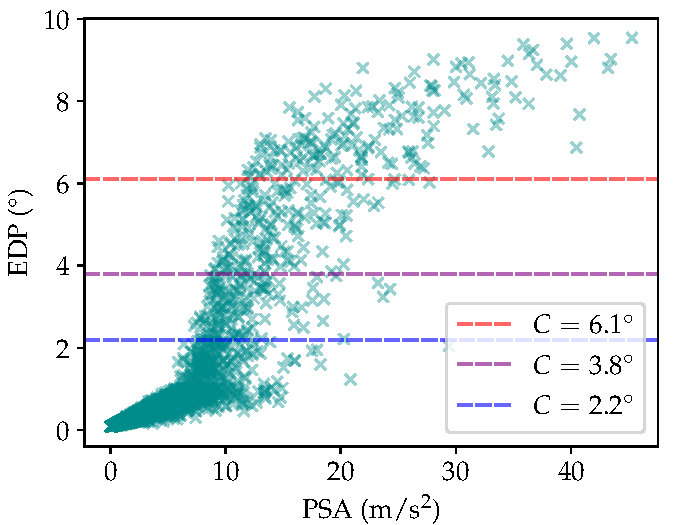
\includegraphics[width=5cm]{figures/DoE/cloud_PSA_light.pdf}\ 
    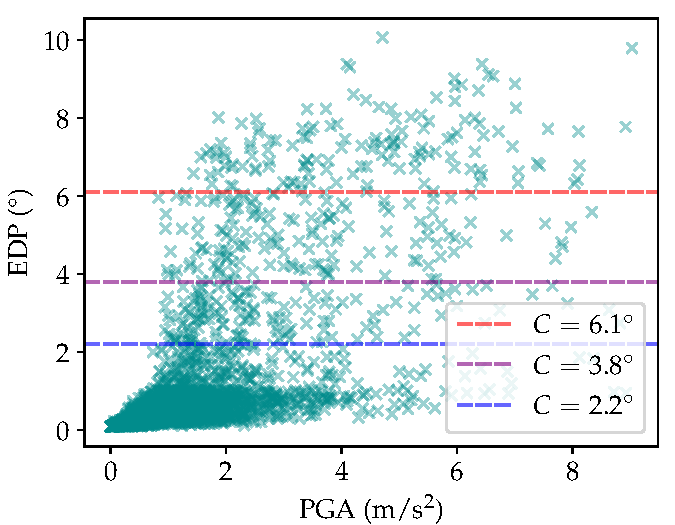
\includegraphics[width=5cm]{figures/DoE/cloud_PGA_light.pdf}%
    % 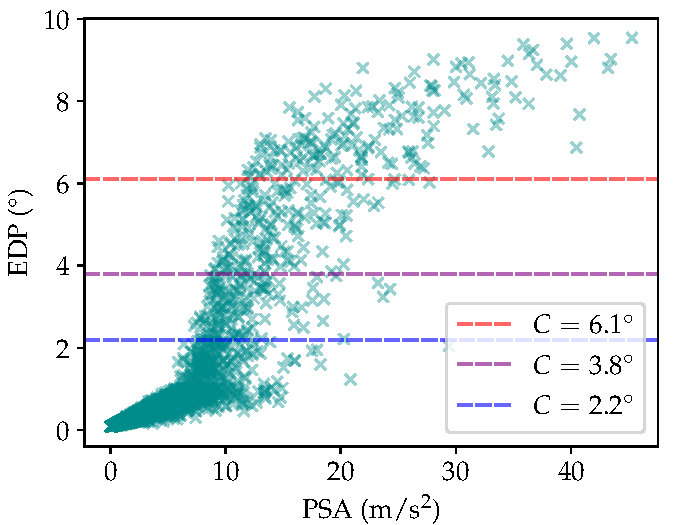
\includegraphics[width=5cm]{figures/DoE/cloud_PSA_light.pdf}%
    % 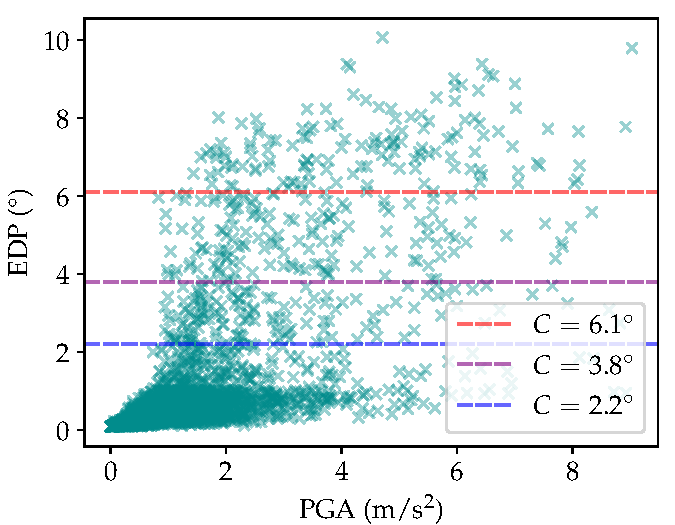
\includegraphics[width=5cm]{figures/DoE/cloud_PGA_light.pdf}%
    \caption{Results of the $8\cdot10^4$ numerical simulations. Each cross is an element of the dataset (IM, EDP) where the IM is the PSA (left) and the PGA (right). Different critical rotation thresholds $C$ are plotted in dashed lines. They yield different proportions of failures in the dataset: respectively 95$\%$ (red), $90\%$ (purple) and $85\%$ (blue).}
    \label{fig:doe:scattersIMs}
    \end{figure}

    \begin{figure}[h!]
        \centering
        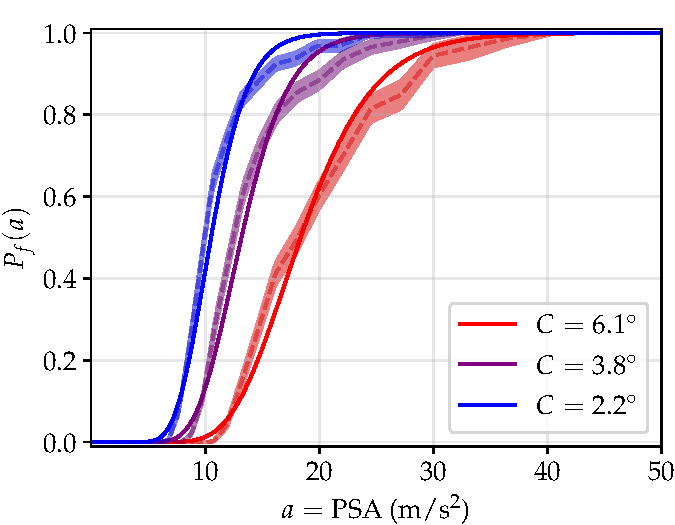
\includegraphics[width=5cm]{figures/DoE/refs_PSA.pdf}\ 
        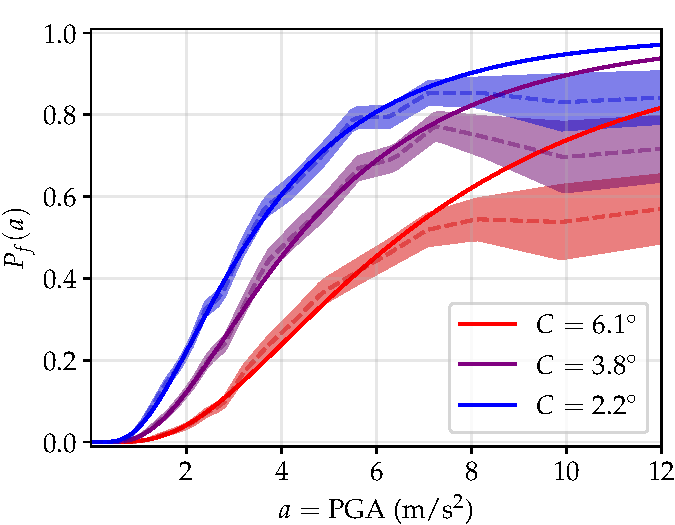
\includegraphics[width=5cm]{figures/DoE/refs_PGA.pdf}
        \caption{{Reference non-parametric fragility curves obtained via Monte Carlo estimates (dashed lines) surrounded by their $95\%$ confidence intervals, for different critical rotation threshold $C$ with (left) the PSA and (right) the PGA as IM.} The thresholds yield different proportions of failures in the dataset: respectively $95\%$ (red), $90\%$ (purple) and $85\%$ (blue).
        For each value of $C$ are plotted (same color, solid line) the corresponding probit-lognormal MLE.}
        \label{fig:doe:reference-frags}
        \end{figure}


    \subsection{Qualitative study}



    In  \cref{fig:doe:ex-estfrag} we present examples of \emph{a posteriori} fragility curve estimations. They take the form of {$95\%$-credibility intervals. These qualitative graphs allow us to appreciate the performance of the estimation when the IMs are selected using our DoE method compared to the standard approach. In this example, the DoE was implemented by setting $\gamma=0.5$.} The same comments stay valid for any of the two IMs we have taken into account in this study ---the PSA and the PGA---, namely: 
    \begin{enumerate}
        \item[(i)] When the number of observed data is really small (20 samples), the standard method tends to provide ``vertical'' fragility curves estimates, which result in ``vertical'' credibility intervals. By verticality, understand here that the tangent of the estimated curve at the median has an infinite slope (i.e., $\beta=0$). This phenomenon is a consequence of the fact that the likelihood is degenerate in this case.
        The credibility intervals are thus tighter but strongly incorrect.
        When the DoE is implemented with the same number of samples, the phenomenon fades and the credibility intervals follow accurately the reference curve.
        \item[(ii)] When a more decent number of data are observed (80 samples), the credibility intervals given from the DoE follow quite closely the reference curve. Within the observed seismic signals, we then notice a better balance between the ones with large IMs and the ones with small IMs compared to the standard method {(see the ``red crosses'' in the figures).} The consequence is a thinner credibility interval given by the DoE method.
        %especially at the borders of the domain.
    \end{enumerate}
    
    \begin{figure}[h]
        \centering%
        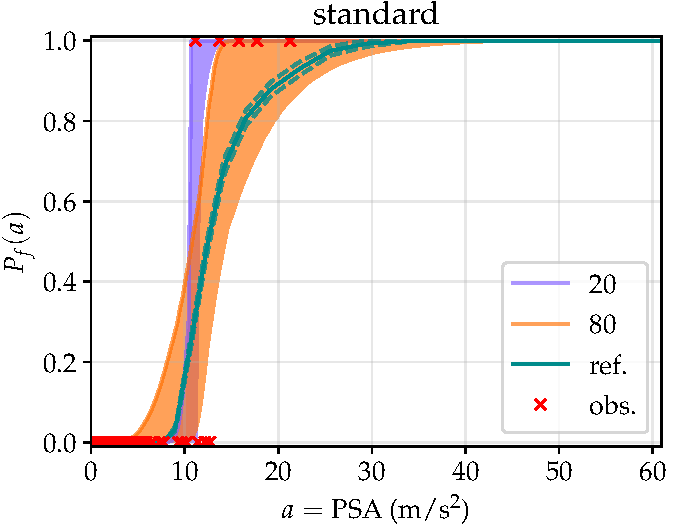
\includegraphics[width=5cm]{figures/DoE/ex_est_frag_PSA_standard_80.pdf}\ %
        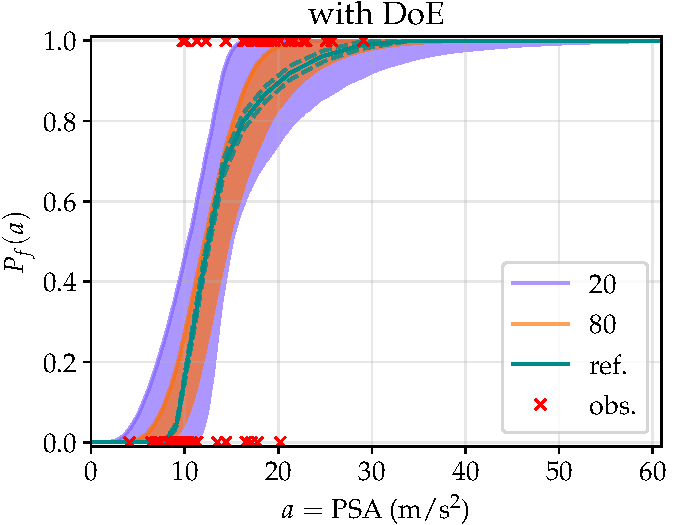
\includegraphics[width=5cm]{figures/DoE/ex_est_frag_PSA_PE_80.pdf}\\[5pt]
        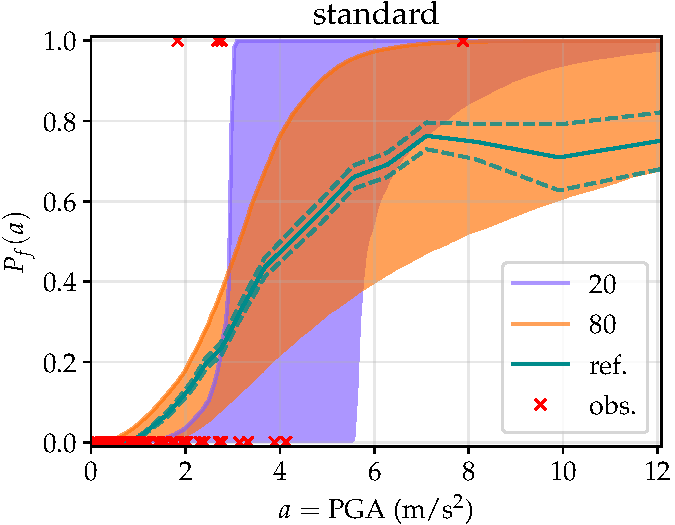
\includegraphics[width=5cm]{figures/DoE/ex_est_frag_PGA_standard_80.pdf}\ 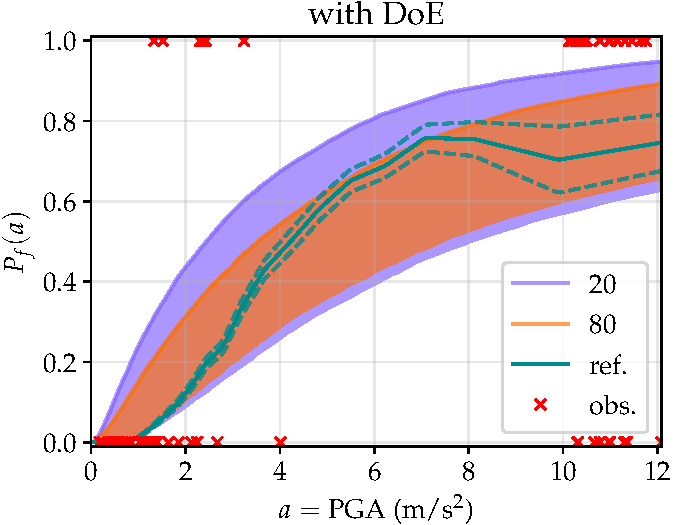
\includegraphics[width=5cm]{figures/DoE/ex_est_frag_PGA_PE_80.pdf}%
        \caption{Examples of fragility curves estimation. Top figures: the IM is the PSA; bottom figures: the IM is the PGA. Left figures: the seismic signals are chosen w.r.t. their standard distribution. Right figures: they are chosen w.r.t. our DoE strategy.
        On each figure: credibility intervals from $20$ (purple) or $80$ (orange) observations, reference fragility curves (green solid line) from Monte Carlo simulations and their {$95\%$}-confidence intervals (green dashed lines). The red crosses represent the $80$ observations.}
        \label{fig:doe:ex-estfrag}
    \end{figure}







    \subsection{Quantitative study}\label{sec:doe:appli:subsec:quantitative}



\Cref{fig:doe:errors-degen,fig:doe:errors-psa,fig:doe:errors-pga,fig:doe:variaI,fig:doe:variaP} present 
quantitative results that go beyond a single example.
Within those, 12 methods are compared:
    the standard method and the DoE methods for any $\gamma\in\{0,$ $0.1,$ $0.3,\dots,1.9\}$.
The case $\gamma=0$ is particular: in this case the prior $\pi^\ast_\gamma$ does not always satisfy the criteria for a robust \emph{a posteriori} estimation (\cref{def:doe:robust-estimation}) even though that is essential for the DoE to be implemented. Thus, $\gamma=0$ corresponds to an alteration of the DoE method:
    first, data are collected given the DoE method carried out with $\gamma=0.1$; second, the prior $\pi^\ast_{0.1}$ is replaced with $\pi^\ast_0$ to compute the estimates.
This particular treatment is carried out in order to quantify how that parametrized constraint affects the estimates.
%This particular variation of the method al

{For each of these methods, we have carried out $100$ replications of the same numerical experiment, namely: (i) generate an observed sample of $k_{\max}=250$ data items and (ii) derive for any $k=10,$ $20,\dots,k_{\max}$ the posterior distribution $p(\theta|\mbf z^k,\mbf a^k)$.
These replications provide evaluations of the mean values of the metrics defined in \cref{sec:doe:metrics}. The results are shown in  \cref{fig:doe:errors-psa} for the PSA and in  \cref{fig:doe:errors-pga} for the PGA.}

%As a first comment, we can compare the results given by the different DoE methods: the errors they give are always very close and we do not clearly distinguish a hierarchization of them w.r.t. the value of $\gamma$. This comment is valid for both the PGA and the PSA. 

\paragraph{{Overall comments on the influence of $\gamma$}}

{For both IMs, \cref{fig:doe:errors-psa,fig:doe:errors-pga} show that the discrepancies between all the DoE-based results are negligible. We do not clearly distinguish a hierarchy of these with respect to the value of $\gamma$.}
We have verified that the selected IMs by the DoE methods are actually poorly influenced by the value of $\gamma$ and that any change of performance impacted by the value of $\gamma$ is hard to distinguish. We conclude that its influence on the posterior estimation remains small. Thus, our constrained reference prior is close enough to the unconstrained ($\gamma = 0$) one and conserves its ``objectivity'' qualification.

\paragraph{Degeneracy disappearance} 

{\Cref{def:degeneracy} lists the different types of situations for which likelihood degeneracy can occur. For our case study,  \cref{fig:doe:errors-degen} presents the average number of occurrences of the three types of situations that lead to a degenerate likelihood, as a function of the number of observed samples. We observe that the DoE method clearly outperforms in reducing the degeneracy for small numbers of observations compared with the standard method (from $k\simeq 20$ in the case of the PGA, and at most $k\simeq 50$ in the case of the PSA). Echoing this observation, we notice that this probability is, in general, higher with the PSA as IM, especially when the seismic signals are selected according to the standard method.

These results must however be qualified because they arise directly from the way in which we implemented the two estimation methods ---DoE and standard---, that is to say from a large database of artificial signals (i.e., of size $8\cdot10^4$), generated {beforehand}. In \cref{app:doe:toycases}, it is indeed  mathematically demonstrated that in a well-specified case, we can define a change of variable between two fragility curves which are defined by two different values of $\theta$, all other things being equal. In other words, from the point of view of the estimation of the parameter $\theta$, all cases are equivalent if there is sufficient data in the domain of interest, that is, the domain in which the fragility curve evolves ``significantly'' from 0 to 1. As this requirement is not met in practice, especially in our case study, the estimation performances are not identical when considering two distinct IMs such as the PGA or the PSA. Thus, in the standard case, whether for the PSA or PGA, as we have considered a high failure threshold, the main cause of degeneracy comes from the fact that the observed data are of type 1, that is to say that they do not reveal any failure. The distributions are concentrated at low IM values. Then, with the PSA, as the value of $\beta$ of the fragility curve is smaller than with the PGA, while its distribution has a larger standard deviation, this favors degeneracy of type 3. To a lesser extent, this also affects the DoE method.}

\begin{figure}[h]
\centering%
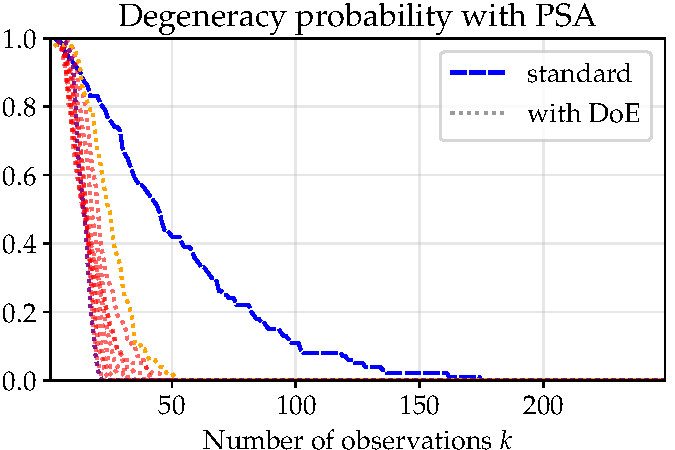
\includegraphics[width=5cm]{figures/DoE/degenPSA.pdf}\ 
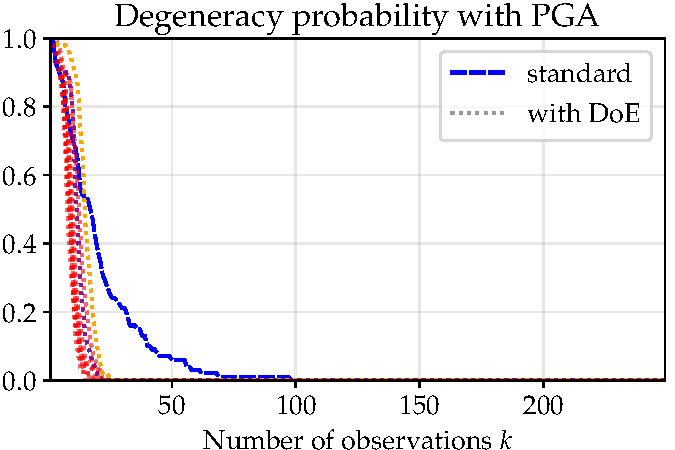
\includegraphics[width=5cm]{figures/DoE/degenPGA.pdf}%
\caption{Probability that a sample of size $k$ yields a degenerate likelihood, as a function of $k$. The considered IM is (left) the PSA and (right) the PGA.
The degeneracy probability without DoE (blue dashed line) is compared with the ones with DoE (dotted lines), for different values of $\gamma$. 
Two extreme values of $\gamma$ are highlighted: $\gamma=0.1$ (purple dotted line) and $\gamma=1.9$ (orange dotted line).}
\label{fig:doe:errors-degen}
\end{figure}


\paragraph{Performances with few observations} {Focusing first on the quadratic errors presented in \cref{fig:doe:errors-psa,fig:doe:errors-pga}, we show that when the number of observations $k$ is small, the outperformance of the DoE method over the standard one is clearly visible for any IM considered.}
Indeed, on the domain $k<50$, the decrease of any of the errors is faster, reaching satisfying values at $k=50$, which is consistent with the qualitative study of the previous section.
Regarding the cases where $k>50$, the behavior of the metrics differ between the case where the PSA is used and the one where it is the PGA. Globally, it is obvious that the PSA provides the best results. The consideration of this IM rather than the PGA is more relevant for this case study. {In the following paragraphs, we discuss more specifically the estimation biases for both IMs, since the quadratic error is a combination of the bias and the credibility width.}

\paragraph{Study of the bias when the IM is the PSA}
As mentioned in \cref{sec:doe:appli:subsec:present}, the PSA is the best of the two IMs in our case study. As a result, the performance of the DoE method is beyond doubt ( \cref{fig:doe:errors-psa}). Up to values of $k$ close to $50$, the decrease in the estimation bias is rapid towards the so-called model bias value which is materialized in the figure (see \cref{sec:doe:metrics}). This bias reflects the fact that the reference fragility curve, $P_f^{\text{ref}}$, does not correspond to an exact probit-lognormal curve as illustrated in  \cref{fig:doe:reference-frags}. Beyond a value of $k$ close to $100$, the bias stops decreasing significantly because it tends towards the model bias. From this threshold, additional observed data only make the credibility intervals thinner around the median. It is noted in this regard that the DoE method is able to provide estimates with a bias that is smaller than the so-called model bias. On average, the DoE-based estimations do not exactly match the model bias, although it is very close. This is not the case for the standard method, for which there is almost an order of magnitude difference, even with a sample size of $250$. The difference between the bias obtained on average by the DoE method and the model bias simply reflects the fact that the distributions of the data used for the estimates are not the same in the two cases. $P_f^{\text{MLE}}$ is estimated on the entire available database while the DoE methodology aims to select some of them by maximizing the criterion defined in \cref{eq:doe:index}. \Cref{app:doe:toycases} provides more insight into the DoE approach.

\begin{figure}[h]
    \centering%
    % \hspace*{-1cm}%
    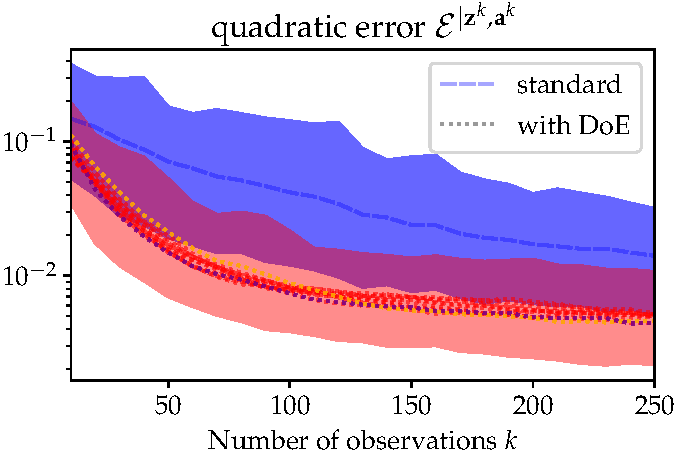
\includegraphics[width=5cm]{figures/DoE/errE_PSA.pdf}\ 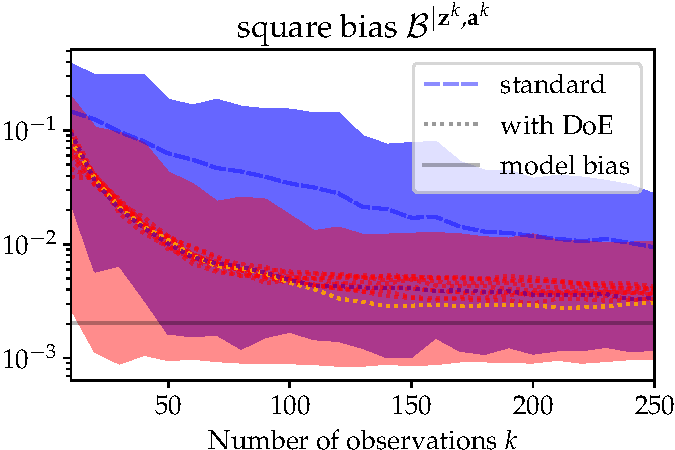
\includegraphics[width=5cm]{figures/DoE/errB_PSA.pdf}\ 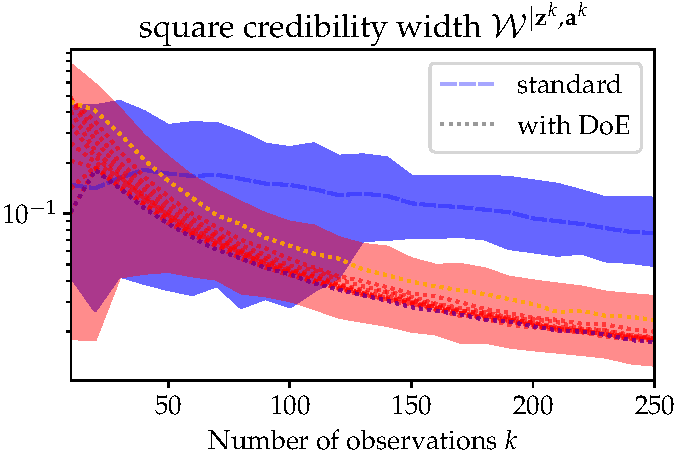
\includegraphics[width=5cm]{figures/DoE/errW_PSA.pdf}%
    \caption{Average error metrics derived from numerous replications of the method, as a function of the size of the observed sample.
    In dashed blue lines: the average errors using the standard distribution of the IM surrounded by their $95\%$-confidence interval. In dotted lines: the average errors using our DoE strategy with different values of $\gamma$. They are surrounded (in red) by the maximal $95\%$-confidence intervals. Two extreme values are emphasized: $\gamma=0$ (orange) and $\gamma=1.9$ (purple).
    On the middle figure, the model square bias is plotted as a gray line.
     The IM  is the PSA here.}
    \label{fig:doe:errors-psa}
\end{figure}



\paragraph{Study of the bias when the IM is the PGA}
{As mentioned in \cref{sec:doe:appli:subsec:present}, with the PGA as IM, it is not possible to fully describe the fragility curve. We therefore have no information on its evolution beyond the maximum value of the PGA observed, at about $12$ m/s$^2$. Moreover, the discrepancies between $P_f^{\text{ref}}$ and $P_f^{\text{MLE}}$ are maximal for a PGA value of the order of $8$ m/s$^2$, whereas before this value the fit is very good.} For the strongest seismic signals at disposal,
equipment failure is only observed in around $70\%$ of cases.
% a failure of the equipment is indeed observed only around {$70\%$} of the time.

{Up to values of $k$ close to $100$, the DoE method outperforms the standard method. Beyond that, the behavior is different from that observed when the IM is the PSA and an evaluation of the performances of the DoE method is less obvious. On average, however, with the first $40$ data points, the bias value obtained with the PGA is smaller than with the PSA.}

%Thus, when $k$ is above $50$, the behavior of the metrics in the case of the PGA ( \cref{fig:errors-pga}) is different {from that observed with PSA}, and an evaluation of the performances of the DoE method in this case is less obvious. Indeed, while the credibility width does not cease to decrease, we notice an increase of the bias that does not stop before $k=150$.

{In \cref{app:doe:toycases} it is shown that with the DoE method, the distribution of the selected data tends to follow 
a bimodal distribution whose modes are equally distant from the logarithm of the median of the fragility curve
% a bimodal distribution equally distributed around the logarithm of the median of the fragility curve 
(see also  \cref{fig:doe:ex-estfrag} and the repartition of the ``red crosses''). Since knowledge of the fragility curve over a restricted domain is likely to reduce the performance of the DoE method, a thorough study of the consequences of such a restriction is proposed in \cref{app:doe:toycases}, in a case where the model bias does not exist. This study shows that the performance of the DoE method is weakly affected by this limitation. We can therefore postulate that it is the presence of a significant bias in one of the two main domains in which the DoE method selects data that is the cause of the deterioration in the method's performance for values of $k > 100$, compared to the standard approach. If we believe the results in  \cref{fig:doe:ex-estfrag}, with $80$ data, we obtain however a completely reasonable estimate, taking into account the observed bias.}

    \begin{figure}[h]
        \centering
        % \hspace*{-1cm}%
        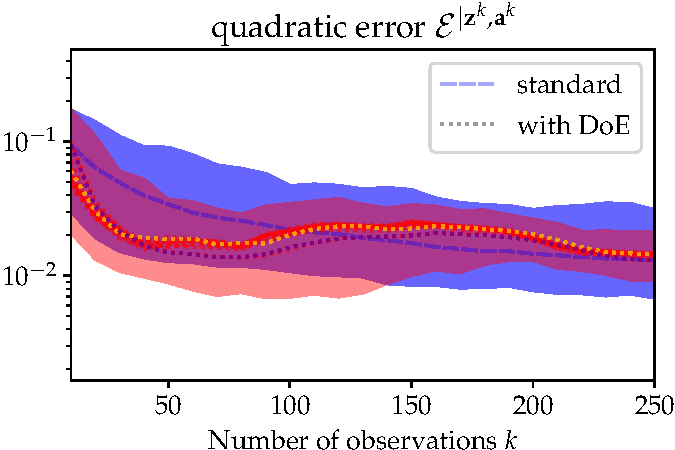
\includegraphics[width=5cm]{figures/DoE/errE_PGA.pdf}\ 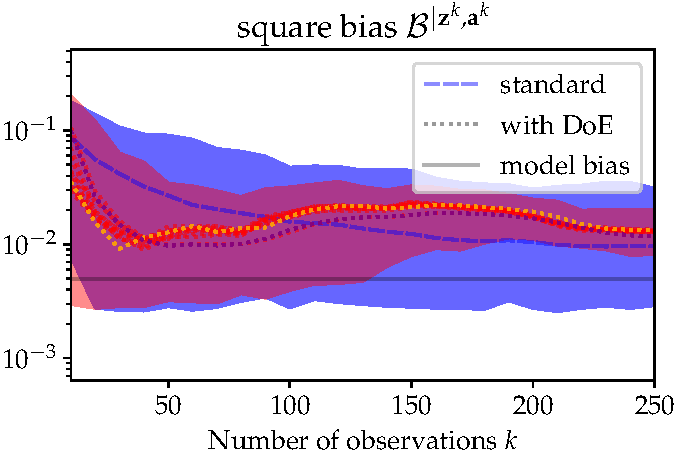
\includegraphics[width=5cm]{figures/DoE/errB_PGA.pdf}\ 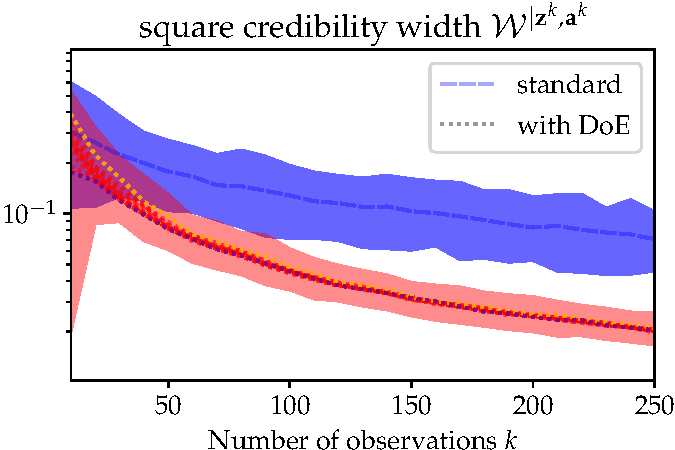
\includegraphics[width=5cm]{figures/DoE/errW_PGA.pdf}%
        \caption{As in \cref{fig:doe:errors-psa} but here the IM  is the PGA.}
       % {Average error metrics derived from numerous replications of the method, as a function of the size of the observed sample. In dashed blue lines: the average errors using the standard distribution of the IM surrounded by their $95\%$-confidence interval. In dotted lines: the average errors using our DoE strategy with different values of $\gamma$. They are surrounded (in red) by the maximal $95\%$-confidence intervals of theirs. Two extreme values are emphasized: $\gamma=0$ (orange) and $\gamma=1.9$ (purple). On the middle figure, the model square bias is plotted as a gray line. The IM considered is the PGA here.}
        \label{fig:doe:errors-pga}
    \end{figure}




    \paragraph{{Stopping criterion}} {To the extent that an irreducible estimation bias can be expected in practice, an indication that such a bias has been reached would constitute a suitable stopping criterion for the DoE method. Since such a criterion would imply knowing, in some way, the bias itself and this is not possible with small data sizes, we suggest to study (i) the index $\cV\cI_k$ that measures the variation of the  quantity defined by \cref{eq:doe:index} that is used to select the seismic signals in the DoE method and (ii) the index $\cV\cP_k$ that measures the average evolution of the median of the fragility curve. These two quantities are defined in \cref{sec:doe:stopping_crit}. They reflect the information provided by adding a $k$-th data point. 

     \Cref{fig:doe:variaI} shows the evolutions of the average values of $\cV\cI_k$ for respectively the PSA and the PGA as IM, whereas  \cref{fig:doe:variaP} is devoted to the evolutions of $\cV\cP_k$. These two figures, once again, show that learning with the DoE method is more effective than with the standard method. $\cV\cI_k$ and $\cV\cP_k$ are slightly influenced by the change in IM. Up to values of $k$ close to $k=50$, they even indicate that with PGA, the DoE method reaches more quickly a state in which the information brought by a new data point has less impact. This result is consistent with the one mentioned in the previous paragraph, namely that with the first $40$ data points, the bias value obtained with the PGA is smaller than with the PSA, with the DoE method.
    
    The practitioner can therefore use these indicators to define a stopping criterion depending on a threshold value. For instance, in our case, a threshold value set at $\cV\cI_k = 10^{-3}$ gives approximately $k_{\max} = 60$ for the PSA and $k_{\max} = 40$ for the PGA. Concerning $\cV\cP_k$, the threshold value can be set at $5 \% $. For both the PSA and the PGA, this ensures furthermore that the likelihood degeneracy probability is zero (see  \cref{fig:doe:errors-degen}). 
    Remark that, even though the number of data required to reach a given stopping criterion is smaller with the PGA than with the PSA, this does not imply that the estimate is less accurate. Indeed, for small data sizes, the degeneracy phenomenon is more likely with the PSA than with the PGA (see  \cref{fig:doe:errors-degen}). Consequently, the widths of the credibility intervals remain large for large $k$ with the PSA (see \cref{fig:doe:errors-psa,fig:doe:errors-pga}). Our approach addresses this phenomenon by reducing the degeneracy even for a few observations. In practice, however, this number remains dependent on the IM of interest (see the paragraph ``Degeneracy disappearance'').
    
    }
        
        %It is interesting to see that its evolution is consistent with the one of the bias: above a certain value of $k$, its decline slows down.
    
            %\begin{equation}
            %    \cI_{k+1}(a_{k+1}) = \EE_{z_{k+1}|\mbf a^{k+1},\mbf z^k}[D_\delta(p(\theta|\mbf z^k,\mbf a^k)||p(\theta|\mbf z^{k+1},\mbf a^{k+1}))],\quad \cV\cI_k = \frac{|\cI_{k+1}(a_{k+1})-\cI_k(a_k)|}{|\cI_k(a_k)|}
            %\end{equation}
        %(see \cref{sec:PEmethod} for the computation of $\cI$). The average value of $\cV\cI_k$ is exhibited in  \cref{fig:variaI}. It is interesting to see that its behavior is consistent with the one of the bias: above a certain threshold value of $k$, its decline slows down. It also matches the average evolution of the fragility curve $\cV\cP_k$ defined by 
           % \begin{equation}
            %    \cV\cP_k = \frac{\|m^{|\mbf z^k,\mbf a^k} - m^{|\mbf z^{k+1},\mbf a^{k+1}}\|_{L^2}}{\|m^{|\mbf z^k,\mbf a^k}\|_{L^2}};
            %\end{equation}
    
        %when the estimated fragility curves cease to clearly evolve, the average information given by new data also does. A stop criterion could be set when $\cV\cI_k$ falls below $10^{-3}$.
        %Indeed, in this case the minimal bias is close to be reached, and additional observations would result into a thinner credibility interval around this bias. It is thus pointless to pursue the experiments as the model bias is irreducible.
    
    
    \begin{figure}[h]
        \centering%
        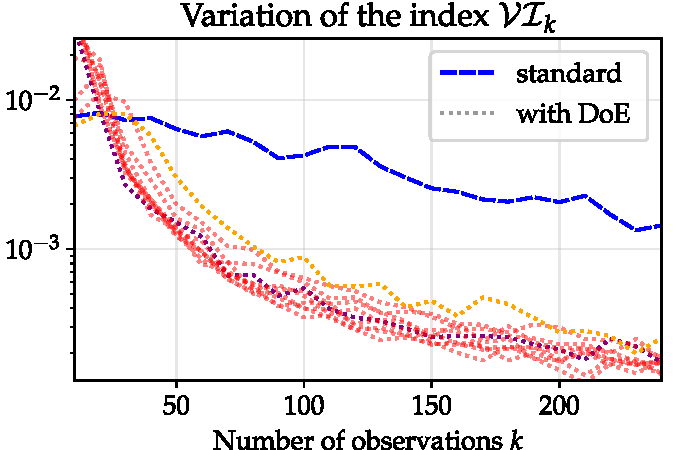
\includegraphics[width=5cm]{figures/DoE/VariaI_PSA.pdf}\ 
        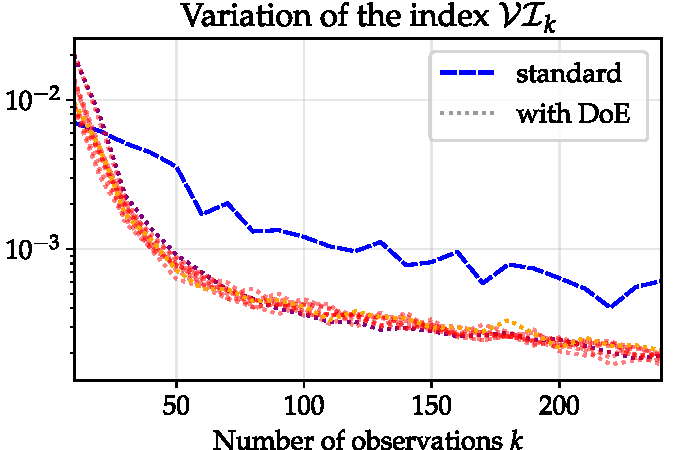
\includegraphics[width=5cm]{figures/DoE/VariaI_PGA.pdf}
        \caption{Average variations of the DoE index $\cV\cI_k$ as a function of the observed sample size $k$, using the PSA (left) and the PGA (right).}
        \label{fig:doe:variaI}
    \end{figure}
    
    
    \begin{figure}[h]
        \centering%
        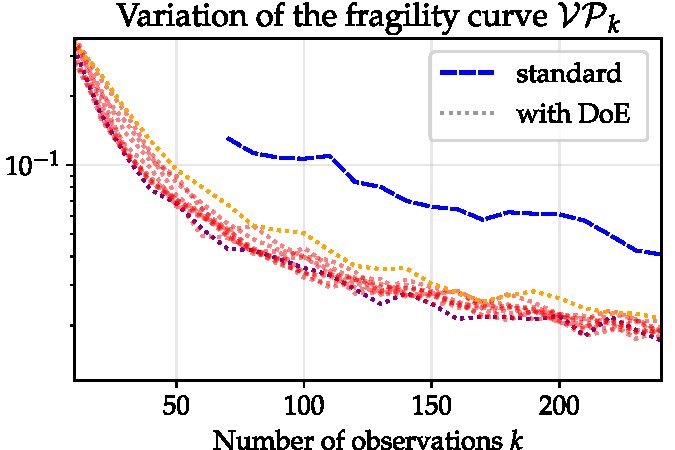
\includegraphics[width=5cm]{figures/DoE/VariaP_PSA.pdf}\ 
        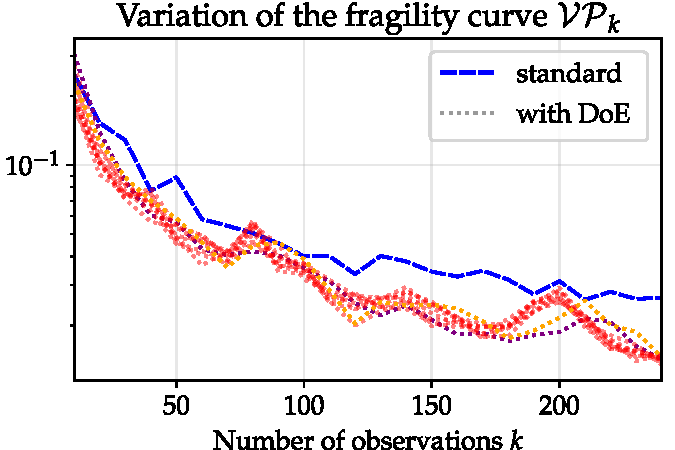
\includegraphics[width=5cm]{figures/DoE/VariaP_PGA.pdf}
        \caption{Average variations of the median \emph{a posteriori} fragility curve $\cV\cP_k$ as a function of the observed sample size $k$, using the PSA (left) and the PGA (right).}
        \label{fig:doe:variaP}
    \end{figure}



    \subsection{Synthesis}




    The objective of the methodology proposed in this work is to make the most of the {probit-}lognormal model. Indeed, it appears to the practitioner as a model that is both pragmatic and relevant for estimating fragility curves with a reduced number of data, judging by the abundant use made of it in the literature. The {limitation} on the number of data is essential. It comes from the fact that (i) these are expensive in absolute terms, especially %with high-fidelity numerical models, or 
with experimental tests, and (ii) the {probit-}lognormal model being likely to be biased, there is no point in feeding it with a lot of data. To achieve this goal, we proposed a methodology for planning experiments in a Bayesian framework based on the reference prior theory.

Two current IMs ---the PSA and the PGA--- were considered to study the performance of the method which was applied to an equipment from the nuclear industry. In both cases, with a few data points ---of the order of 80---, the performance of the proposed method was much better than that of the standard one. Performance is best if the method is used with an IM that has a good level of correlation with the structural response of interest.

In order to guide the user, we also proposed two indicators that allow learning to be stopped based on quantitative information. Both criteria appeared sensitive to the change of IM and therefore to the associated potential biases. Let us add, however, that since the degeneracy phenomenon does not make the estimation optimal from the point of view of the size of the credibility interval, it is appropriate, in practice, to continue learning until a non-degenerate sample is obtained (see \cref{def:degeneracy}).



\section{Behavior of the method on toy case studies}\label{app:doe:toycases}

    \subsection{Description of the case studies}
    

    In order to gain more insight on the method, we suggest in this section a brief analysis of its behavior on case studies that are free of any bias. 
    Such case studies are purely theoretical, so that we qualify them as ``toy case studies''. Here, the observed data $(\mbf z^k,\mbf a^k)$ are perfectly generated according to the probit-lognormal statistical model presented in \cref{sec:doe:model}:
    a reference parameter $\theta^\ast=(\alpha^\ast,\beta^\ast)$ is chosen; then, from any input $a$ (that simulates a theoretical IM), an output $z\in\{0,1\}$ is generated that is equal to $1$ with probability $\Phi\left(\beta^{\ast -1}\log\frac{a}{\alpha^{\ast}}\right)$ and $0$ otherwise.
    
    The selected inputs belong to an interval $\cA=(0,a_{\text{max}}]$.
    They are picked by the {design} of experiments methodology that we present in this work with $\gamma=0.5$. Note that when implementing \cref{alg:doe:PE} in this section, there is no need to generate seismic signals from a particular value of $a$ here. Indeed, the ``experiment'' (understand here: the generation of $z$) directly results from $a$.
    Regarding the $k_0=2$ required initial values of $a$, we draw them uniformly in $\cA$.
    
    In those toy case studies, the value of $\theta^\ast$ does not matter, in the sense that two such case studies with two different value of $\theta^\ast$ would be equivalent up to a translation and a dilatation w.r.t. $\log a$ (see \cref{app:equiv-toy} for a proof of this statement).
    
    In this section, we present three different toy case studies. They are all implemented using the same value of $\theta^\ast$. 
    They differ from the different domains $\cA$ that are selected for them.
    The limits $a_{\text{max}}$ of these domains are chosen to simulate an upper bound 
    on the possible IM that can result from a generated seismic signal.
    They are selected to match a quantile of the reference fragility curve: if $q\in[0,1]$ one can derive $a_q$ such that $P^{\text{ref}}_f(a_q):=\Phi\left(\beta^{\ast -1}\log\frac{a_q}{\alpha^{\ast}}\right)=q$, i.e.
        \begin{equation}
            a_q = \exp\left( \beta^\ast t_q+\log\alpha^\ast \right),
        \end{equation}
    where $t_q$ represents the $q$-quantile of a standard Gaussian distribution.
    
    The three toy case studies implemented in this work result from defining $a_{\text{max}}=a_q$ with:
    \begin{itemize}
        \item $q\simeq1$ (actually $q=1-10^{-3}$), to represent a case where no upper bound (or a very high one regarding the fragility curve) limits the generation of IMs. %This case could correspond to the scale of the case study of \cref{sec:application} when the IM is the PSA (however, there are no bias here).
        \item $q=0.9$.
        \item $q=0.8$.
    \end{itemize}
    The reference fragility curve of each of these toy case studies are plotted in  \cref{fig:histograms_toy} (green solid lines) for each of the values of $q$ aforementioned, and for $\theta^\ast=(3,0.3)$. 
    %On  \cref{fig:ex_est_toys} are presented examples of credibility interval estimation.
    
    
    
    
    
    \subsection{Results}
    
    The design of experiments method has been replicated a hundred times for each case study. Each time, we have stopped the algorithm after it reached a number of $250$ observed samples.
    The last $100$ of these generated IMs have been kept for each replication. As we have carried out $100$ replications, they constitute a sample of $10^4$ values of IMs selected by the experimental design.
    %To focus on the distribution of the selected IMs by the method, we kept for each  the 100 last ones. Thus, we have at our disposal a sample of $10^4$ values of IMs selected by the planning of experiments algorithm at least 150 steps after its initialization, for each case study. 
    The three empirical distributions of these samples resulting from the three values of $q$ are compared in  \cref{fig:histograms_toy}.
    
    % As one c
    
    When the method is not limited by any upper bound for the choice of IMs (i.e. case $q=1$), 
    the logarithms of the selected ones are symmetrically distributed around $\log\alpha^\ast$. This comment was expected as in the statistical modeling, $\log a$ is mathematically symmetric around $\log\alpha^\ast$ as well.
    
    The bimodal appearance of the distribution supports the ``well-posedness'' of the method. Indeed, in a case where the result is deterministic, the knowledge of the evaluation of the curve in two points is enough to recover its parameter $\theta^\ast$. Thus, it makes sense that the optimal distribution of the IM for estimating the whole fragility curve is to retrieve a proper estimation of its evaluation in two zones of the domain.
    A simple calculation is done in \cref{sec:au-maths-calc} to suggest possible appropriate centers of the zones. 
    {These are called $a^u_1$ and $a^u_2$ and are appropriate in the sense that they are the points that most help distinguish a stochastic fragility curve from a deterministic one.}
    %two different fragility curves.}
    %they are optimal in the sense that they are the {points} where the estimated value of the fragility curve is expected to be the worse when it is compared with the reference. {!!  je vais y réflechir mais cette phrase n'est pas très clair à mon sens !!}
    In  \cref{fig:histograms_toy}, their values are emphasized (dashed pink line). They are clearly close from the actual modes of the empirical distribution of the IM in the case $q=1$.
    
    
    In the cases where the IM selection is limited ($q<1$), the method has been designed to select $a_{\text{max}}$ when the index tended to be maximized by a value which is higher.
    We notice that the method seems to target the same ideal domain as when $q=1$: converging to a bimodal strategy with modes around optimal domains. The method is robust: for two given $q_1$, $q_2$ and their $a_{\text{max}}^1$, $a_{\text{max}}^2$, associated to two toy case studies, around the same proportion of IMs is selected below $a$ for any $a\leq\min(a_{\text{max}}^1, a_{\text{max}}^2)$ in the two cases.
    This results in numerously selected IMs equaling $a_{\text{max}}$ when it falls close to the second expected mode of the optimal distribution.
    
    In  \cref{fig:metrics-toy}-left, we compare the average square bias
    resulting from the 100 replications of the three case studies.
    Their difference is difficult to distinguish, so the robustness of the method is confirmed: even when the limit among the available IMs sharply intersects  the reference fragility curve, the distribution of the selected ones still provides an accurate estimation.
    However, a close look allows to notice the expected loss of performance induced by such limit: the smaller is $q$, the larger is the bias.
    
    Regarding the other metrics exposed in  \cref{fig:metrics-toy}, namely the indices $\cV\cI_k$ and $\cV\cP_k$, it is interesting to notice that their behaviors are comparable to that of the real case study. In particular, $\cV\cI_k$ reaches the threshold $10^{-3}$ for a similar number of observations (around $50$) in any of the case studies implemented in this work (real ones as well as toy ones).
    As a matter of fact, the index sequentially measures the quantity of information brought by the next seismic signal selected by the DoE. Thus, the stability of that quantity between case studies supports the robustness of our approach in selecting IMs to inform the estimate and enhance the learning.
    However, the indices $\cV\cP_k$ are smaller for toy case studies. Without any model bias, the estimates reach more quickly the reference (see the average bias in  \cref{fig:metrics-toy}-left), so that they evolve less.
    
    %{
    %Finally, this section helps to clarify the limit of a comparison between the results obtained with two different IMs in \cref{sec:quantitative-study}. 
    %Indeed, a clear difference between the cases where the IM is the PGA and the one where it is the PSA is the difference of scale of the reference fragility curve between those two. When it is the PGA, the fragility curve is cut far before being close to one, when it equals around $0.8$ or $0.9$. 
    %Thus, up to the model bias, an analogy is possible between the real case studies and the toy ones, where the piping system with PSA corresponds to our toy case study with $q=1$, and the piping system with PGA corresponds to $q=0.8$ or $q=0.9$. 
    %The results elucidated in this section prove that this difference has little influence on the estimates by deteriorating slightly the square bias. This deterioration remains however negligible in front of the model biases of the real case studies.}
    
    {Finally, this section helps to clarify the results obtained with the two IMs that are the PSA and the PGA in \cref{sec:doe:appli:subsec:quantitative}. The main difference between them is that with the PGA it is not possible to completely describe the fragility curve. With the PGA, the maximum value of its probit-lognormal estimate is approximately $0.8$ but does not reach $1$ as with the PSA. If we ignore the bias, this means that the case $q=1$ is similar to the situation where the PSA is used as IM, while the cases  $q=0.8$ and $q=0.9$ are similar to the situation where the PGA is used. All things being equal, this study shows that the performance of the DoE method is weakly affected by a restricted learning domain. It is then likely that the presence of a significant bias in one of the two main domains in which the DoE method selects data is the cause of its performance degradation.}
    
    %
    %As proven by the results elucidated in this section, a short upper bound on the IM influences the estimation with a higher bias. This coincides with comments done in \cref{sec:quantitative-study}. However, as precised in the above paragraph, the impact of this phenomenon on the bias remains really little. That confirms that in the case of the piping system, the variations of the bias when the PGA is used as IM resorts to multiple factors. {!! il me semble qu'il faudrait reprendre ce dernier paragraphe car il manque de clarté, même si à demi-mot on comprend ce que tu veux dire !!}
    
    \begin{figure}[h]
            \centering%
            % \makebox[0pt][c]{%}
            %\hspace*{-2cm}
            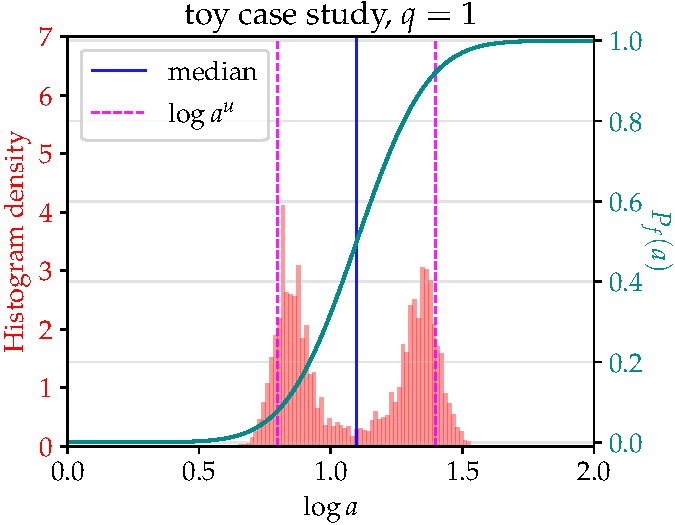
\includegraphics[width=5cm]{figures/DoE/toy_A_1.pdf}\ 
            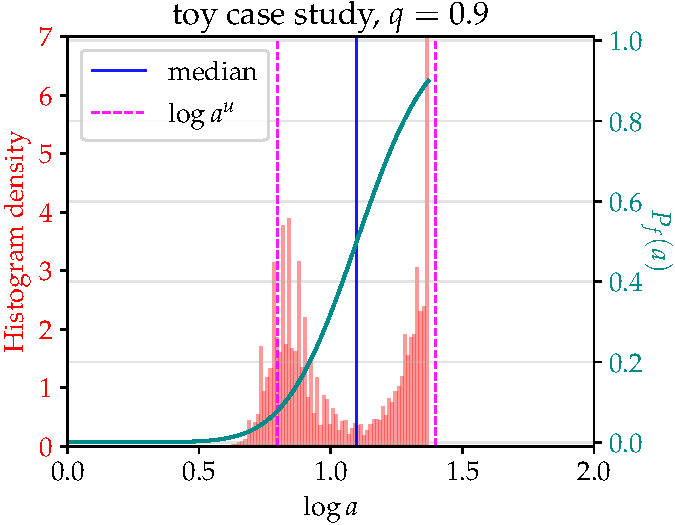
\includegraphics[width=5cm]{figures/DoE/toy_A_09.pdf}\ 
            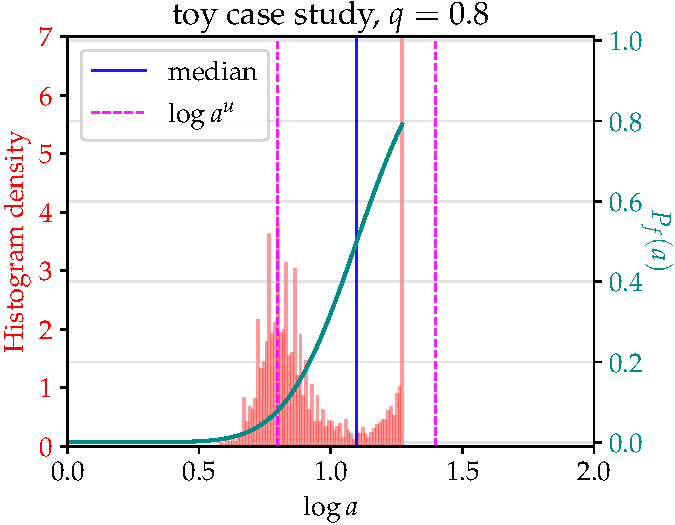
\includegraphics[width=5cm]{figures/DoE/toy_A_08.pdf}%}%
            \caption{For each of the three toy case studies: the distribution of the 100 last selected IM by the method (red histograms) along with the associated reference fragility curve (green) of the toy case study, which is cut at a certain quantile $q$ in each figure. The median of the reference (solid blue) and the values $a^u_{1}$, $a^u_{2}$ (dashed pink) are emphasized.}
            \label{fig:histograms_toy}
        \end{figure}
    
    % \begin{figure*}
    %         \centering%
    %         \makebox[0pt][c]{%}
    %         %\hspace*{-2cm}
    %         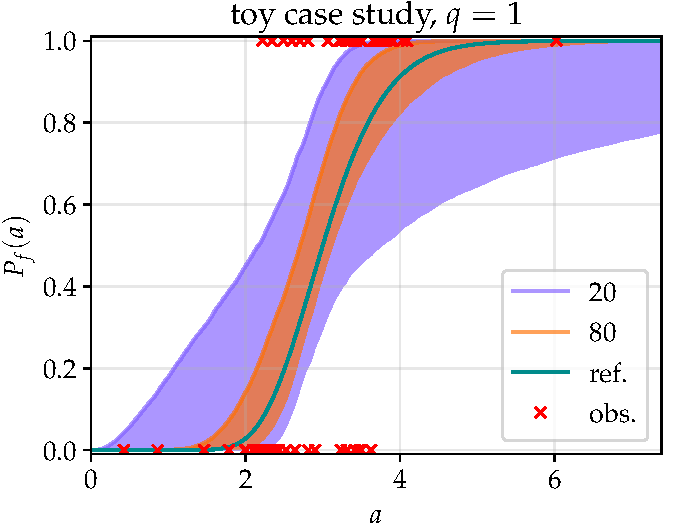
\includegraphics[width=5cm]{figures/ex_toy_1.pdf}\ 
    %         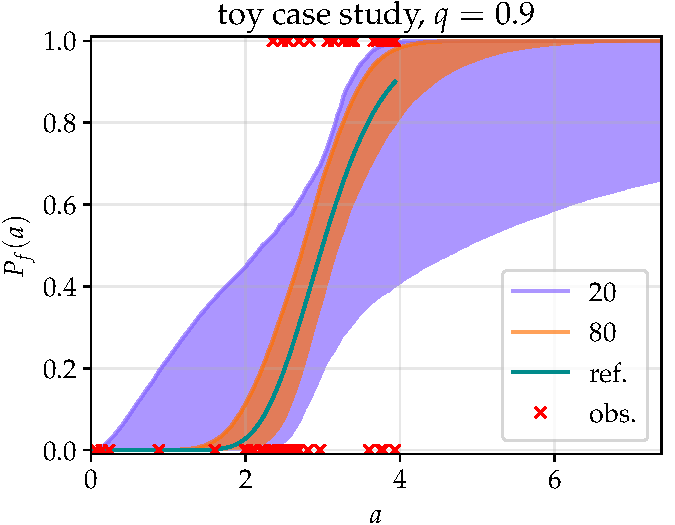
\includegraphics[width=5cm]{figures/ex_toy_09.pdf}\ 
    %         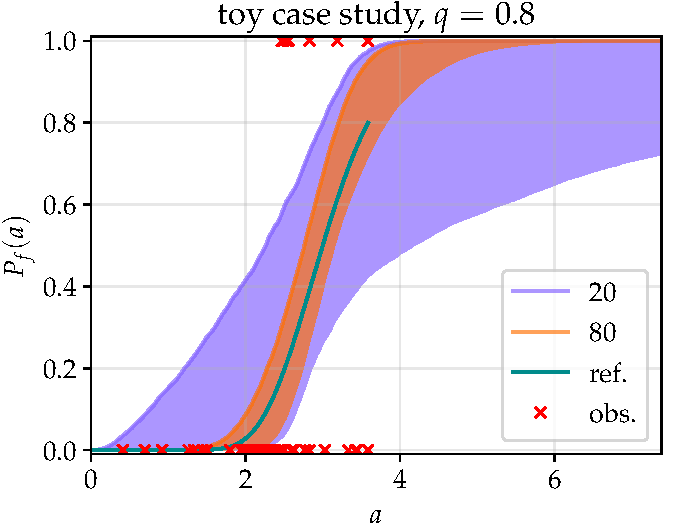
\includegraphics[width=5cm]{figures/ex_toy_08.pdf}}%
    %         \caption{Examples of credibility intervals estimation for each of the three toy case studies. On each case, 80 observed data (red crosses) have been selected via the DoE method. The \emph{a posteriori} credibility intervals are derived for 20 of the observed samples (in purple), and for the 80 ones (in orange). On each case, the reference (green) is cut from $a_{\max}$. Note that any comparison is limited because the distribution of selected data remains volatile (especially for 20 samples).}
    %         \label{fig:ex_est_toys}
    %     \end{figure*}
    
    
        % \begin{figure}
        %     \centering
        %     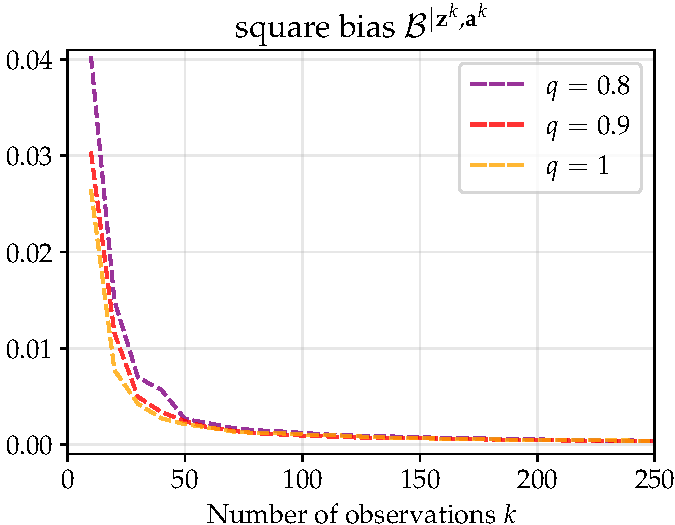
\includegraphics[width=5cm]{figures/toy_bias.pdf}
        %     \caption{Average square bias of the three toy case studies as a function of the number of observations.}
        %     \label{fig:bias-toy}
        % \end{figure}
    
    \begin{figure}[h]
        \centering%
        % \makebox[0pt][c]{%}
        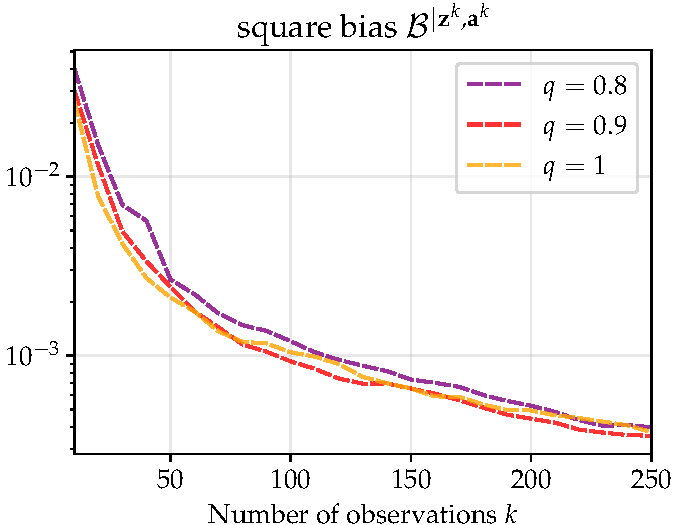
\includegraphics[width=5cm]{figures/DoE/toy_bias_log.pdf}%
        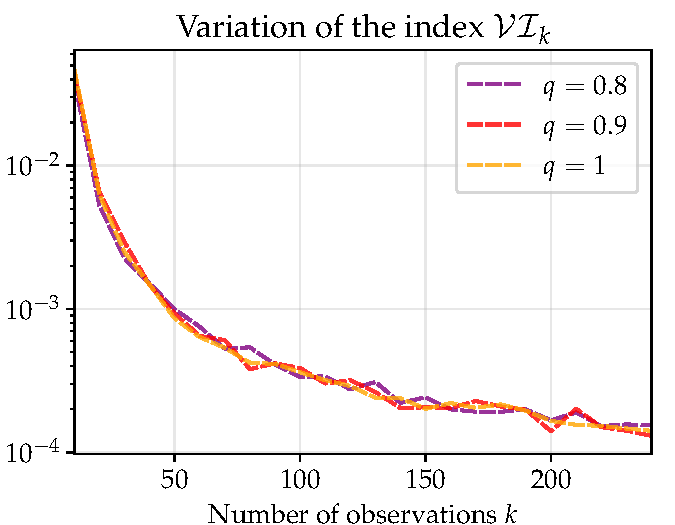
\includegraphics[width=5cm]{figures/DoE/toyVI.pdf}%
        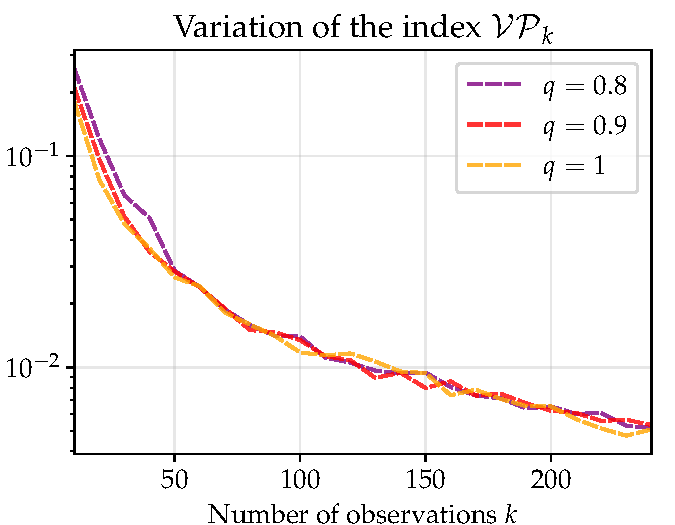
\includegraphics[width=5cm]{figures/DoE/toyVP.pdf}%}%
        \caption{Left figure: average square bias of the three toy case studies as a function of the number of observations. Middle figure: index $\cV\cI_k$ for the three toy case studies as a function of the number of observations. Right figure: index $\cV\cP_k$ for the three toy case studies as a function of the number of observations.}
        \label{fig:metrics-toy}
    \end{figure}
    
    
    
    \subsection{Simple suggestion of a domain where IMs should be theoretically selected}\label{sec:au-maths-calc}
    
    
    
    
    In this section we suggest a criterion that gives insight on a domain where the
    fragility curve should be evaluated in order to optimize the estimation.
    {For this purpose, we study the quantity $\EE[ |P^{\text{ref}}_f(a)-P_f(a)| ]$ as a function of $a$, where $P^{\text{ref}}_f(a)$ represents a deterministic fragility curve and $P_f(a)$ denotes a stochastic estimate.
    If $a^\ast$ is a maximal argument of this quantity, it would 
    be the one that helps the most distinguishing the two curves.}
    %represent the best point to compare the fragility curves in order to discriminate them
    %A maximal argument of this quantity would 
    %give points within which the distinction between }
    %be a value of the IM within which the expected estimation is the worse, i.e. an input where there is a lack of information. 
    %Additional evaluations of the output in this point should thus enhance the most the evaluation.
    
    
    
    
    
    For this theoretical study, we assume to be in the settings of the toy case studies defined in the previous subsection, i.e. $P^{\text{ref}}_f(a)=\Phi\left(\beta^{\ast -1}\log\frac{a}{\alpha^{\ast}}\right)$ for a couple $(\alpha^\ast,\beta^\ast)$.
    We derive
        \begin{align}\nonumber
            &\frac{d}{da}\EE|P^{\text{ref}}_f(a)-P_f(a)|\\ &= \frac{1}{a\sqrt{2\pi}}\int_\Theta \left[\frac{1}{\beta^\ast}\exp\left(-\frac{(\log a-\log\alpha^\ast)^2}{2\beta^{\ast 2}}\right)-\frac{1}{\beta} \exp\left(-\frac{(\log a-\log\alpha)^2}{2\beta^2}\right)\right] p_{\alpha,\beta}(\alpha,\beta)d\alpha d\beta. \label{eq:derive-P-EP}   
        \end{align}
    To pursue, we can assume that $(\alpha,\beta)$ follows an inverse-gamma-normal distribution. This class covers a wide range of different distributions and is conjugate with a normal distribution, so that the following computation is tractable. Additionally, the probit-lognormal modeling of the fragility curve is equivalent to assume that there exists a latent variable $Y$ that is linearly correlated with the input: $Y=\log A +\cN(-\log\alpha^\ast,\beta^\ast)$. Considering this latent modeling, we can prove that both the reference prior and the posterior distribution of $\alpha,\beta$ belong to the class of inverse-gamma-normal ones (see \cref{app:chap:ESAIM}).
        %
    % If we consider the least informative case for $p_{\alpha,\beta}$ where $\log\alpha$ has an uniform distribution on $\RR$, then the left-hand term of \cref{eq:derive-P-EP}) is equal to
    %     \begin{equation}
    %         \frac{1}{\sqrt{2\pi}}\frac{1}{a\beta^\ast}\exp\left(-\frac{(\log a-\log\alpha^\ast)^2}{2\beta^{\ast2}}\right) - \frac{1}{a},
    %     \end{equation}
    % which equals $0$ if and only if $a=a^u_1$ or $a=a^u_2$ where the latter are defined by 
    %     \begin{equation}
    %         a^u_{1,2} = \alpha^\ast\exp\left( \pm\sqrt{2}\beta^\ast \left|\log\beta^\ast\sqrt{2\pi} \right|^{1/2} \right).
    %     \end{equation}
    %
    % In a more general case than the least informative one, we can assume $(\alpha,\beta)$ to follow an inverse-gamma-lognormal distribution. Indeed, such a distribution (i) remains general enough to cover a lot of possible distributions, (ii) is conjugate with a normal distribution so that the computation stays tractable. Moreover, the probit-lognormal modeling is equivalent to assume that a latent variable $Y$ is linearly correlated with the input : $Y=\log a+\cN(-\log\alpha^\ast,\beta^2)$, $Z$ being equal to $\indic_{Y>0}$.
    % Considering this latent modeling, both the reference prior and the posterior distribution of $\alpha,\beta$ belong to inverse-gamma-lognormal ones \cite{VanBiesbroeckESAIMProcS}. 
    The inverse-gamma-lognormal distribution is defined by its density:
    \begin{align}
        p_{\alpha,\beta}(\alpha,\beta) &= K(c,d,\tau,\zeta)\left(\frac{1}{\beta^2}\right)^{c+1/2}\exp\left(-\frac{d}{\beta^2}\right)\exp\left(-\tau\frac{(\log\alpha-\zeta)^2}{2\beta^2}\right),\nonumber\\
        \text{with}\quad K(c,d,\tau,\zeta) &=\frac{d^c\sqrt{\tau}}{\Gamma(c)\sqrt{2\pi}},
    \end{align}
    where $c>0$, $d>0$, $\tau>0$ and $\zeta\in\RR$ are the parameters of the distribution. %Note that the non-informative settings treated previously corresponds to the limit case where $\tau=0$.
    
    Thus, the right-hand term in  \cref{eq:derive-P-EP} becomes:
    \begin{equation}
        \frac{1}{\sqrt{2\pi}}\frac{1}{a\beta^\ast}\exp\left(-\frac{(\log a-\log\alpha^\ast)^2}{2\beta^{\ast2}}\right) - \frac{d^c}{(d+\frac{\tau}{2\tau+2}(\zeta-\log a)^2)^{c+1/2}}\frac{\sqrt{\tau}}{\sqrt{\tau+1}}\frac{\Gamma(c+\frac{1}{2})}{\Gamma(c)}\frac{1}{a\sqrt{2\pi}},
    \end{equation}
    so that it equals $0$ if and only if $a$ verifies:
    \begin{equation}\label{eq:equality-au}
        |\zeta-\log a|\frac{e^{1/2}}{\beta^\ast}\exp\left(-\frac{(\log a-\log\alpha^\ast)^2}{2\beta^{\ast2}}\right) = \frac{d^c|\zeta-\log a|e^{1/2} }{(d+\frac{\tau}{2\tau+2}(\zeta-\log a)^2)^{c+1/2}}\frac{\sqrt{\tau}}{\sqrt{\tau+1}}\frac{\Gamma(c+\frac{1}{2})}{\Gamma(c)}.
    \end{equation}
    Given the derivations conducted in \cref{app:additionalmaths}, the right-hand term of the above equation tends to 1 when information is provided by observed data to the posterior. In this case and if $\zeta=\log\alpha^\ast$  the equation leads to $a=a^u_1$ or $a=a^u_2$ where $a^u_1$, $a^u_2$ are defined by
        \begin{equation}
            a^u_{1,2} = \alpha^\ast\exp\left(\pm\beta^\ast\right).
        \end{equation}
    
    These values are built on a criterion that has a concrete and practical sense. However, they remain purely theoretical as they depend on the exact value of $\theta^\ast$.
    
    
    
    % Else, it 
    
    
    
    
    % % with the right hand term of 
    % the derivation conducted in Section   states that the right-hand term of the above equation is bounded between 
    
    
    \subsection{Additional mathematical derivations}\label{app:additionalmaths}
    
        The goal of this section is to study the domain of the right-hand term of \cref{eq:equality-au}, especially in the ``worst'' cases (the distribution is very-informative or non-informative).
        We rely on the following lemmas:
        \begin{lem}\label{lem:app-ineqG}
            For any $c>0$, $\displaystyle{\frac{\Gamma\left(c+\frac{1}{2}\right)}{\Gamma(c)}<\sqrt{c}}$. Also, $\displaystyle{
                \lim_{c\rightarrow\infty}\frac{\Gamma\left(c+\frac{1}{2}\right)}{\Gamma(c)\sqrt{c}}=1.
                }$
        \end{lem}
        \begin{proof}
            The first statement is a direct consequence of Gautschi's inequality \citep{gautschi_elementary_1959}: for any $c>0$, $s\in(0,1)$,
                \begin{equation}
                    c^{1-s}<\frac{\Gamma(c+1)}{\Gamma(c+s)}<(c+1)^{1-s}.
                \end{equation}
            Fixing $s=1/2$ and using the identity $\Gamma(c+1)=c\Gamma(c)$ leads to the result.
    
            For the second statement, we can rely on Stirling's formula \citep{davis_leonhard_1959} that yields:
                \begin{equation}
                    \Gamma(c+t) \equi{c\rightarrow\infty} \Gamma(c)c^t
                \end{equation}
            for any $t\in\CC$.
        \end{proof}
        
        \begin{lem}\label{lem:app-ineqdcf}
            Let $f>0$, for any $d,c>0$ we define:
            \begin{equation}
                g(c,d) = \frac{\sqrt{c}}{(d+f)^{1/2}}\left(\frac{d}{d+f}\right)^c, \quad h(d) = \frac{1}{2}\log\left(1+\frac{f}{d}\right)^{-1}.
            \end{equation}
            Thus, for any $c,d>0$, $g(c,d)<(2ef)^{-1/2}$, and $\displaystyle{\lim_{d\rightarrow\infty}g(h(d),d)=(2ef)^{-1/2}}.$
        \end{lem}
        \begin{proof}
            Let us differentiate $g$ w.r.t. $c$:
            \begin{equation}
                \frac{\partial}{\partial c}g(c,d) = (d+f)^{-1/2}\left(\frac{d}{d+f}\right)^c\left[\sqrt{c}\log\left(\frac{d}{d+f}  \right)+\frac{1}{2\sqrt{c}}\right].
            \end{equation}
            The above quantity is decreasing w.r.t. $c$ and equals $0$ when $c=h(d)$.
            We deduce that for any $d>0$, 
            \begin{equation}\label{eq:lem:ghdd}
                g(c,d)<g(h(d),d) = \frac{(2e)^{-1/2}}{(d+f)^{1/2}}\log\left(1+\frac{f}{d}\right)^{-1/2}.
            \end{equation}
            
            Now, let us briefly study the function $v(t)=(1+t^{-1})\log(1+t)$ for $t>0$.
            Firstly, $\log(1+t)\equi{t\rightarrow0}t$ so that $v(t)\conv{t\rightarrow0}1$. Secondly, $v'(t) = \frac{1}{t}-\frac{1}{t^2}\log(1+t)$, which is positive for any $t>0$, and tends to $\frac{1}{2}$ when $t=0$. Therefore, $v(t)>v(0)=1$ for any $t>0$. 
    
            Going back to \cref{eq:lem:ghdd}, we can write $g(h(d),d)=(2ef)^{-1/2}v(f/d)^{-1/2}$ to obtain that
                \begin{equation}
                    g(c,d) <(2ef)^{-1/2}\quad\text{and} \quad \lim_{d\rightarrow\infty}g(h(d),d)=(2ef)^{-1/2}.
                \end{equation}
        \end{proof}
    
    The result of \cref{lem:app-ineqdcf} with $f=\frac{1}{2}\frac{\tau}{\tau+1}(\log a-\zeta)^2$ lets us write the following inequality:
        \begin{equation}
            \frac{d^c\sqrt{c}}{(d+\frac{\tau}{2\tau+2}(\zeta-\log a)^2 )^{c+1/2}}\frac{\sqrt{\tau}}{\sqrt{\tau +1}} < \frac{e^{-1/2}}{|\zeta-\log a|},
        \end{equation}
        this upper-bound being reached at the boundary of the domain. Combining this statement with \cref{lem:app-ineqG}, we obtain: 
            \begin{equation}
                \frac{d^c|\zeta-\log a|e^{1/2}}{(d+\frac{\tau}{2\tau+2}(\zeta-\log a)^2 )^{c+1/2}}\frac{\sqrt{\tau}}{\sqrt{\tau +1}}\frac{\Gamma(c+\frac{1}{2})}{\Gamma(c)} < 1,    
            \end{equation}
        this upper-bound being reached at the boundary of the domain.
    
        Additionally, the left-hand term of the above equation is non-negative and tends to $0$ for some extreme values of the parameters.
        Therefore, there exist two extreme cases for the resolution of \cref{eq:equality-au}: when its right-hand term equals $0$ and when it equals $1$. The former corresponds to the limit case where the solution is $a=\pm\infty$ or $a=\zeta$, with $a=\pm\infty$ minimizing the quantity of interest. 
        The latter corresponds to the limit case where the solution verifies
            \begin{equation}
                \frac{|\zeta-\log a|^2}{\beta^{\ast2}} = \exp\left( \frac{|\log\alpha^\ast-\log a|^2}{\beta^{\ast2}} -1\right).
            \end{equation}
        The solutions of the above equation when $\zeta =\log\alpha^\ast$ are $a=\alpha^\ast\exp\left(\pm\beta^\ast\right).$
        They correspond to the limit case when the distribution $p_{\alpha,\beta}$ becomes informed and unbiased. 
        If the model is appropriately specified, that should be the fate of the posterior distribution: the posterior tends to match a normal distribution with mean $\theta^\ast$ and variance $\frac{1}{k}\cF^{-1}(\theta^\ast)$ where $\cF$ refers to the Fisher information matrix \citep{van_der_vaart_asymptotic_1992}.
    
        
    
    
    
    
    \subsection{Equivalence between toy case studies}\label{app:equiv-toy}
    
        Let us consider two different toy case studies. They can differ by their reference parameters $\theta_1^\ast$, $\theta_2^\ast$ and their IMs $a_1$, $a_2$, which are defined in the domains $\cA_1$, $\cA_2$.
        We suppose that the bounds of $\cA_1$ and $\cA_2$ are defined to match the same quantiles of the reference fragility curves: $\cA_1=(c_1^1,c_1^2)$, $\cA_2=(c_2^1,c_2^1)$ with $P^{\mathrm{ref}}_1(c_1^1)=P^{\mathrm{ref}}_2(c_2^1)$ and $P^{\mathrm{ref}}_1(c_1^2)=P^{\mathrm{ref}}_2(c_2^2)$, where $P^{\mathrm{ref}}_1$ (reps. $P^{\mathrm{ref}}_2$) denotes the reference fragility curves given by $\theta_1^\ast$ (resp. $\theta^\ast_2$).
    
        Therefore, if we introduce $\tilde a$ that defines the value of a new IM on the second toy case study, which verifies
        \begin{equation}
            \log\tilde a = \frac{\log c_1^2-\log c_1^1}{\log c_2^2-\log c_2^1}\log\frac{a_2}{c_2^1} + \log c_1^1,
        \end{equation}
        we obtain that $\tilde a$ lives in the domain $\tilde\cA=\cA_1$. Given this new IM, the reference fragility curve of the second case study can be re-defined as a function of $\tilde a$:
            \begin{equation}
                \tilde P^{\mathrm{ref}}_2(\tilde a) = \Phi\left(\beta^{\ast-1}_2\left[\frac{\log c_2^2-\log c_2^1}{\log c_1^2-\log c_1^1}\left(\log\tilde a-\log c_1^1\right)+\log c_1^1-\log\alpha^\ast_2 \right]\right) = \Phi\left(\tilde\beta^{\ast-1}_2\log\frac{\tilde a}{\tilde\alpha^\ast_2}\right),
            \end{equation}
        for a certain $\tilde\theta^\ast_2 = (\tilde\alpha_2^\ast,\tilde\beta_2^\ast)$.
        We have $\tilde P^{\mathrm{ref}}_2(c_1^1)=P^{\mathrm{ref}}_2(c_2^1)=P^{\mathrm{ref}}_1(c_1^1)$ and $\tilde P^{\mathrm{ref}}_2(c_1^2)=P^{\mathrm{ref}}_2(c_2^2)=P^{\mathrm{ref}}_1(c_1^2)$, thus, as the parameter $\theta$ defines uniquely a probit-lognormal fragility curve, $\theta_1=\tilde\theta_2$.
    
        As a conclusion, given a rescaling of the IM, the two case studies are equivalent.
    
        
    
% \section{Application of the method on the piping system}


% \subsection{Case study description as a reminder}


% \subsection{}


\section{Conclusion}\label{sec:doe:conclusion}





% In some sense, this chapter can be seen as an ``ultimate'' application 





% Assessing 
% the estimation of probit-lognormal seismic fragility curves in a Bayesian framework
% amounts to 


When we seek to estimate seismic fragility curves with limited data, 
the information conveyed by any sources ---the prior, the observations, the model--- have a considerable influence on the quality of estimates.


%the seismic fragility of structures and components 
%when few binary data are available ---i.e., less than 100--- is a challenging task. To do this, it is often necessary to introduce some simplifying assumptions. 
%The simplest and most widespread assumption assumes a linear correlation between the logarithm of the structural response of interest and the logarithm of the IM of interest. However, recent studies have shown that this assumption should be avoided because of the unavoidable bias it may introduce, which can greatly affect the estimation. Another preferred solution in the literature, 
%A standard solution found in the literature
%is to use a parametric model of the fragility curves such as the probit-lognormal model. This is the choice that was made in this work.

%Several methods can be implemented to estimate the model parameters. Th the use of Bayesian methods which are known to be regularizing. The question of the choice of the prior is then significant because it inevitably impacts all the resulting estimates, especially with small data sizes.

In this work, we considered as in the previous chapters the probit-lognormal model, and had thus to acknowledge its irreducible bias compared with the actual reference fragility curves of the studied component.
%limited

Regarding \emph{a priori} information, we 
relied on the reference prior theory in order to define the prior. This framework makes it possible to define a so-called objective prior in the sense that it favors the information brought by the data to the estimates. Because the
most objective prior according to the theory does not
tackle degenerate likelihoods and issues improper posteriors, we derived a slightly modified reference prior, more efficient and more robust.
However, one has to note that this prior is slightly more informative than the original reference prior.

To optimize data allocation, we have proposed a design of experiments strategy that also inherits from the reference prior theory, i.e., that is based on information theory. Given a large database of synthetic seismic signals, the proposed strategy intends to sequentially select the synthetic signals with which to perform the calculations or the tests, in order to optimally estimate ---by minimizing their number--- the probit-lognormal estimations of fragility curves.

We proved that our method is robust and
that \emph{a priori} information incorporated through the modified prior is quickly negligible in front of the information brought by the data when they are selected by the experimental design.
Compared to a standard approach that aims to select seismic signals in their initial distribution, considering the Jeffreys prior, we have shown the superiority of our method. It allows reaching more quickly ---i.e., with a limited number of data--- a small estimation bias with a small credibility interval, while reducing the phenomenon of degeneracy. The proposed methodology therefore makes the most of the log-normal model. Since estimation biases can be expected in practice, it is recommended to use the method with few data (i.e., less than 100). To this end, we propose two stopping criteria that reflect the information provided by any additional data.
\newpage
% Finally, let us note that the DoE methodology was applied here within the framework of the reference prior theory because the authors believe that the objectivity of the prior is essential for fragility analyses. However, the DoE methodology can be applied with any prior that is proper.


